\documentclass[11pt]{article}
%\documentclass[11pt,draft]{article}   % uncomment this and comment out the above line for *fast* typesetting (no images)


\usepackage{endnotes}
\usepackage{float}


\usepackage{fancybox}
\usepackage{graphicx}
\usepackage{amsmath}
\usepackage{amsfonts}
\usepackage{amssymb}
\usepackage{amsthm}

\usepackage{url}
\DeclareMathOperator{\Li}{Li}
\DeclareGraphicsRule{.tif}{png}{.png}{`convert #1 `dirname #1`/`basename #1 .tif`.png}

\newcommand{\mycaption}[1]{\begin{quote}{\bf Figure: } \large #1\end{quote}}

\newcommand{\ill}[3]{ 
   \begin{figure}[H]
   \begin{center}
   \includegraphics[width=#2\textwidth]{illustrations/#1}
   \caption{#3}
   \end{center}
    \end{figure}
}

\newcommand{\illtwo}[4]{ 
   \begin{figure}[H]
   \begin{center}
   \includegraphics[width=#3\textwidth]{illustrations/#1}$\qquad$\includegraphics[width=#3\textwidth]{illustrations/#2}
   \caption{#4}
    \end{center}
    \end{figure}
}

\newcommand{\illthree}[5]{ 
   \begin{figure}[H]
   \begin{center}
   \includegraphics[width=#4\textwidth]{illustrations/#1}$\qquad$\includegraphics[width=#4\textwidth]{illustrations/#2}$\qquad$\includegraphics[width=#4\textwidth]{illustrations/#3}
   \caption{#5}
    \end{center}
    \end{figure}
}

%%%% Theoremstyles
\theoremstyle{plain}
\newtheorem{theorem}{Theorem}[section]
\newtheorem{proposition}[theorem]{Proposition}
\newtheorem{corollary}[theorem]{Corollary}
\newtheorem{claim}[theorem]{Claim}
\newtheorem{lemma}[theorem]{Lemma}
\newtheorem{hypothesis}[theorem]{Hypothesis}
\newtheorem{conjecture}[theorem]{Conjecture}

\theoremstyle{definition}
\newtheorem{definition}[theorem]{Definition}
\newtheorem{question}[theorem]{Question}
\newtheorem{problem}[theorem]{Problem}
\newtheorem{alg}[theorem]{Algorithm}
\newtheorem{openproblem}[theorem]{Open Problem}

%\theoremstyle{remark}
\newtheorem{goal}[theorem]{Goal}
\newtheorem{remark}[theorem]{Remark}
\newtheorem{remarks}[theorem]{Remarks}
\newtheorem{example}[theorem]{Example}
\newtheorem{exercise}[theorem]{Exercise}

\numberwithin{equation}{section}
\numberwithin{figure}{section}
\numberwithin{table}{section}


\textwidth = 6.5 in
\textheight = 9 in
\oddsidemargin = 0.0 in
\evensidemargin = 0.0 in
\topmargin = 0.0 in
\headheight = 0.0 in
\headsep = 0.0 in
\parskip = 0.2in
\parindent = 0.0in


\def\GL{\mathrm{GL}}
\def\PGL{\mathrm{PGL}}
\def\PSL{\mathrm{PSL}}
\def\GSP{\mathrm{GSP}}
\def\Z{\mathrm{Z}}
\def\Q{\mathrm{Q}}
\def\Gal{\mathrm{Gal}}
\def\Hom{\mathrm{Hom}}
\def\Ind{\mathrm{Ind}}
\def\End{\mathrm{End}}
\def\Aut{\mathrm{Aut}}
\def\loc{\mathrm{loc}}
\def\glob{\mathrm{glob}}
\def\Kbar{{\bar K}}
\def\D{{\mathcal D}}
\def\L{{\mathcal L}}
\def\R{{\mathcal R}}
\def\G{{\mathcal G}}
\def\W{{\mathcal W}}
\def\H{{\mathcal H}}
\def\OH{{\mathcal OH}}


\title{What is Riemann's Hypothesis?}
\author{Barry Mazur \and William Stein}

\begin{document}

\maketitle
\tableofcontents

\section{\label{foreword}Foreword}

\bigskip

The Riemann Hypothesis is one of the great unsolved problems of
mathematics and the reward of \$1,000,000 of {\em Clay Mathematics
  Institute} prize money awaits the person who solves it. But---with
or without money---its resolution is crucial for our understanding of
the nature of numbers.

There are at least four full-length books recently published, written
for a general audience, that have the Riemann Hypothesis as their main
topic.  A reader of these books will get a fairly rich picture of the
personalities engaged in the pursuit, and of related mathematical and
historical issues.\endnote{List these four books here with some discussion of each?}
     
This is {\em not} the mission of the booklet that you now hold in your
hands. We aim---instead---to explain, in as direct a manner as
possible and with the least mathematical background required, what
this problem is all about and why it is so important. For even before
anyone proves this {\em hypothesis} to be true (or false!), just
getting familiar with it and with some of the the ideas behind it, is
exciting.  Moreover, this hypothesis is of crucial importance in a
wide range of mathematical fields; for example it is a
confidence-booster for computational mathematics: even if the Riemann
Hypothesis is never proved, its truth gives us an excellent sense of
how long certain computer programs will take to run, which, in some
cases, gives us the assurance we need to initiate a computation that
might take weeks or even months to complete.

      
Our ``booklet'' comes in two pieces: the actual text which is a mere
\pageref{lastpage} pages, and a web page ({\tt
  http://rh.publisher...}) which has a gallery of illustrations that
are meant to accompany the text.  There are very few mathematical
equations in our text.  But for the more adventurous readers, we have
also included at the above website something we call {\em worksheets}
that explain to the reader how to experiment with the parameters for
the ranges of data illustrated, so as to get a vivid sense of how the
numbers ``behave.''
 
\ill{riemann}{.3}{Bernhard Riemann (1826--1866)}

So, what {\em is} the Riemann Hypothesis? Here is a {\em first
  description} of this hypothesis, put in one ridiculously condensed
paragraph. We will be giving other quite miraculous formulations of
this hypothesis as well; the task of our booklet is to expand the
following paragraph into a real {\em explanation} and to convince you
of its importance and its beauty.
      
      \begin{center}
       \shadowbox{ \begin{minipage}{0.9\textwidth}
\mbox{}       \vspace{0.2ex}
       \begin{center}{\bf\large What {\em sort} of Hypothesis is the Riemann Hypothesis?}\end{center}
       \medskip

Consider the seemingly innocuous series of questions:

\begin{quote}
How many prime numbers  (2, 3, 5, 7, 11, 13, 17, … ) are there less than 100?\\
How many less than 10,000?\\
How many less than 1,000,000?\vspace{-1ex}\\

More generally, how many primes are there less than any given number $X$?
\end{quote}

Riemann proposed, a century and half ago, a strikingly
simple-to-describe ``very good approximation'' to the number of
primes less than a given number $X$. We now
see that if we could prove this {\em Hypothesis of Riemann} we would have
the key to a wealth of powerful mathematics. Mathematicians are eager
to find that key.


\vspace{1ex}
\end{minipage}}
      \end{center}
      
\begin{figure}[H]\label{fig:bott}
\begin{center}
% I got this from http://www.math.harvard.edu/history/bott/
% Barry says there  is a good picture in the book
% "the Index Theorem" that Yau published.
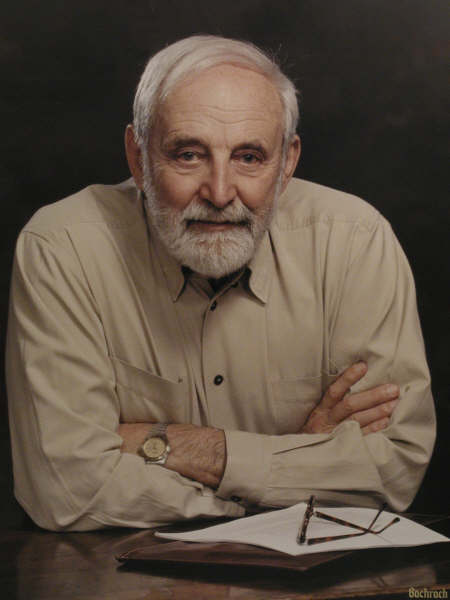
\includegraphics[width=0.3\textwidth]{illustrations/raoulbott}
\caption{Raoul Bott (1923--2005)}
\end{center}
\end{figure}

A famous mathematician, Raoul Bott (see Figure~\ref{fig:bott}), once
said---giving advice to some young mathematicians---that whenever one
reads a mathematics book or article, or goes to a math lecture, one
should aim to come home with something very specific (it can be small,
but should be {\em specific}) that has application to a wider class of
mathematical problem than was the focus of the text or lecture.  If we
were to suggest some possible {\em specific} items to come home with,
after read our booklet, three key phrases -- {\bf prime numbers}, {\bf
  square-root accurate}, and {\bf error term} -- would head the
list. As for words of encouragement to think hard about the first of
these, i.e., prime numbers, we can do no better than to quote a
paragraph of Don Zagier's classic 12-page exposition, {\em The First
  50 Million Prime Numbers}:
    
\begin{quote}                      
  ``There are two facts about the distribution of prime numbers of
  which I hope to convince you so overwhelmingly that they will be
  permanently engraved in your hearts. The first is that, [they are]
  the most arbitrary and ornery objects studied by mathematicians:
  they grow like weeds among the natural numbers, seeming to obey no
  other law than that of chance, and nobody can predict where the next
  one will sprout. The second fact is even more astonishing, for it
  states just the opposite: that the prime numbers exhibit stunning
  regularity, that there are laws governing their behavior, and that
  they obey these laws with almost military precision.''
\end{quote}
                    
\begin{figure}[H]\label{fig:zagier}
\begin{center}
% I took this myself when we were hiking in Oberwolfach once...
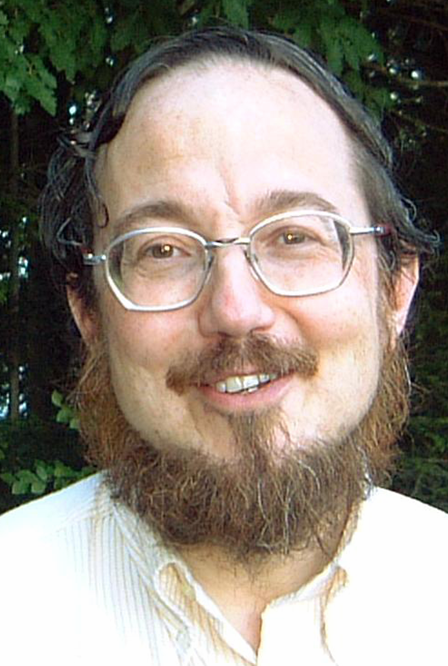
\includegraphics[width=0.25\textwidth]{illustrations/zagier}
\caption{Don Zagier}
\end{center}
\end{figure}

\section{Thoughts about numbers: ancient, medieval, and modern}

If we are to believe the ancient Greek philosopher Aristotle the early
Pythagoreans thought that the principles governing Number are ``the
principles of all things,'' the concept of Number being more basic than
{\em earth, air, fire, or water}, which were according to ancient tradition
the four building blocks of matter. To think about number is to get
close to the architecture of ``what is.''

So, how far along are we in our thoughts about numbers?

The French philosopher and mathematician Ren\'e Descartes, almost four
centuries ago, expressed the hope that there soon would be ``almost
nothing more to discover in geometry.'' Contemporary physicists dream
of a final theory\endnote{Link to Weinberg's book {\em Dreams of a
    Final Theory: The Search for the Fundamental Laws of Nature}, by
  Steven Weinberg (New York: Pantheon Books, 1992)}.  But despite its
venerability and its great power and beauty, the pure mathematics of
numbers may still be in the infancy of its development, with depths to
be explored as endless as the human soul, and never a final theory.


% This is from http://en.wikipedia.org/wiki/File:Frans_Hals_-_Portret_van_Ren%C3%A9_Descartes.jpg
% There is a higher resolution scan available there

\ill{descartes}{.3}{Ren\'e Descartes}


\ill{dulcinea1.jpg}{.2}{Don Quixote and ``his'' Dulcinea del Toboso}

Numbers are obstreperous things. Don Quixote encountered this when he
requested that the ``bachelor'' compose a poem to his lady Dulcinea del
Toboso, the first letters of each line spelling out her name. The
``bachelor'' found

\bigskip


\begin{quote}
  ``a great difficulty in their composition because the number of
  letters in her name was $17$, and if he made four Castilian stanzas
  of four octosyllabic lines each, there would be one letter too many,
  and if he made the stanzas of five octosyllabic lines each, the ones
  called {\em d{\'e}cimas} or {\em redondillas,} there would be three
  letters too few...''
\end{quote}
  
``It must fit in, however, you do it,'' pleaded Quixote, not willing to
grant the imperviousness of the number $17$ to division.

% http://www.jus.uio.no/sisu/don_quixote.miguel_de_cervantes/60.html#2068

\bigskip


{\em Seventeen} is indeed a prime number: there is no way of factoring
it as the product of smaller numbers, and this accounts---people tell
us---for its occurrence in some phenomena of nature, as when
the $17$-year cicadas all emerged to celebrate a ``reunion'' of some
sort in our fields and valleys.

\ill{cicada}{.3}{Cicadas emerge every 17 years}
% from http://biology.clc.uc.edu/steincarter/cicadas.htm

\bigskip


Prime numbers, despite their {\em primary} position in our modern
understanding of number, were not specifically doted over in the
ancient literature before Euclid, at least not in the literature that
has been preserved. Primes are mentioned as a class of numbers in the
writings of Philolaus (a predecessor of Plato); they are not mentioned
specifically in the Platonic dialogues, which is surprising 
given the intense interest Plato had in mathematical developments; and
they make an occasional appearance in the writings of Aristotle, which
is not surprising, given Aristotle's emphasis on the distinction
between the {\em composite} and the {\em incomposite}. ``The
incomposite is prior to the composite,'' writes Aristotle in Book 13 of
the Metaphysics.
[[By prior does he mean ``more important than'' or ``comes before''?  I.e., is the quote
really saying ``The incomposite is more important than and comes before the composite.''
I ask, because the word prior as above is definitely not everyday modern
plane-spoken English, and I don't want to trip up our readers unnecessarily.  A
short endnote or rephrasing or maybe a different translation could really help here.
This might be a good opportunity to cite your Imagining Numbers book.]]
           
\bigskip


But, until Euclid, prime numbers seem not to have been singled out as
{\em the} extraordinary mathematical concept, central to any deep
understanding of numerical phenomena, that they are now understood to
be.
       
\bigskip


There is an extraordinary wealth of established truths about numbers;
these truths provoke sheer awe for the beautiful complexity of prime
numbers. But each of the important new discoveries we make give rise
to a further richness of questions, educated guesses, heuristics,
expectations, and unsolved problems.
            
            \bigskip
            
\section{What are prime numbers?}
            

\noindent {\em Primes as atoms. } To begin from the beginning, think
of the operation of multiplication as a bond that ties numbers
together: the equation $2\times 3= 6$ invites us to imagine the number
$6$ as (a molecule, if you wish) built out of its smaller constituents
$2$ and $3$.  Reversing the procedure, if we start with a whole
number, say $6$ again, we may try to factor it (that is, express it as
a product of smaller whole numbers) and, of course, we would
eventually, if not immediately, come up with $6 = 2\times 3$ and
discover that $2$ and $3$ factor no further; the numbers $2$ and $3$,
then, are the indecomposable entities (atoms, if you wish) that
comprise our number.  By definition, a {\bf prime number}
(colloquially, {\em a prime}) is a whole number, bigger than $1$, that
cannot be factored into a product of two smaller whole numbers. So,
$2$ and $3$ are the first two prime numbers. The next number along the
line, $4$, is not prime, for $4= 2\times 2$; the number after that,
$5$, is. Primes are, multiplicatively speaking, the building blocks
from which all numbers can be made. A fundamental theorem of
arithmetic tells us that any number (bigger than $1$) can be factored
as a product of primes, and the factorization is {\em unique} except
for rearranging the order of the primes. 

For example, if you try to factor the number $12$ as a product of
smaller numbers---ignoring the order of the factors---there are two
ways to begin to do this:
$$
  12 = 2 \times 6 \qquad\text{ and }\qquad   12 = 3 \times 4
$$
But neither of these ways is a full factorization of $12$, for both
$6$ and $4$ are not prime, so can be themselves factored, and in each
case after changing the ordering of the factors we arrive at:
$$
   12= 2 \times 2 \times 3.
$$

If you try to factor the number $300$, there are many
ways to begin:
$$
  300= 30\times 10\qquad\text{or}\qquad 300 = 6 \times 50
$$
and there are various other starting possibilities. But if you continue the factorization (``climbing down'' any one of 
the possible ``factoring trees'') to the bottom, where every factor is a prime number, e.g., in
Figure~\ref{fig:factor300},
you always end up with the same collection of prime numbers:                  
                 $$300 = 2^2\times 3\times 5^2.$$   

\begin{figure}[H]
\begin{center}
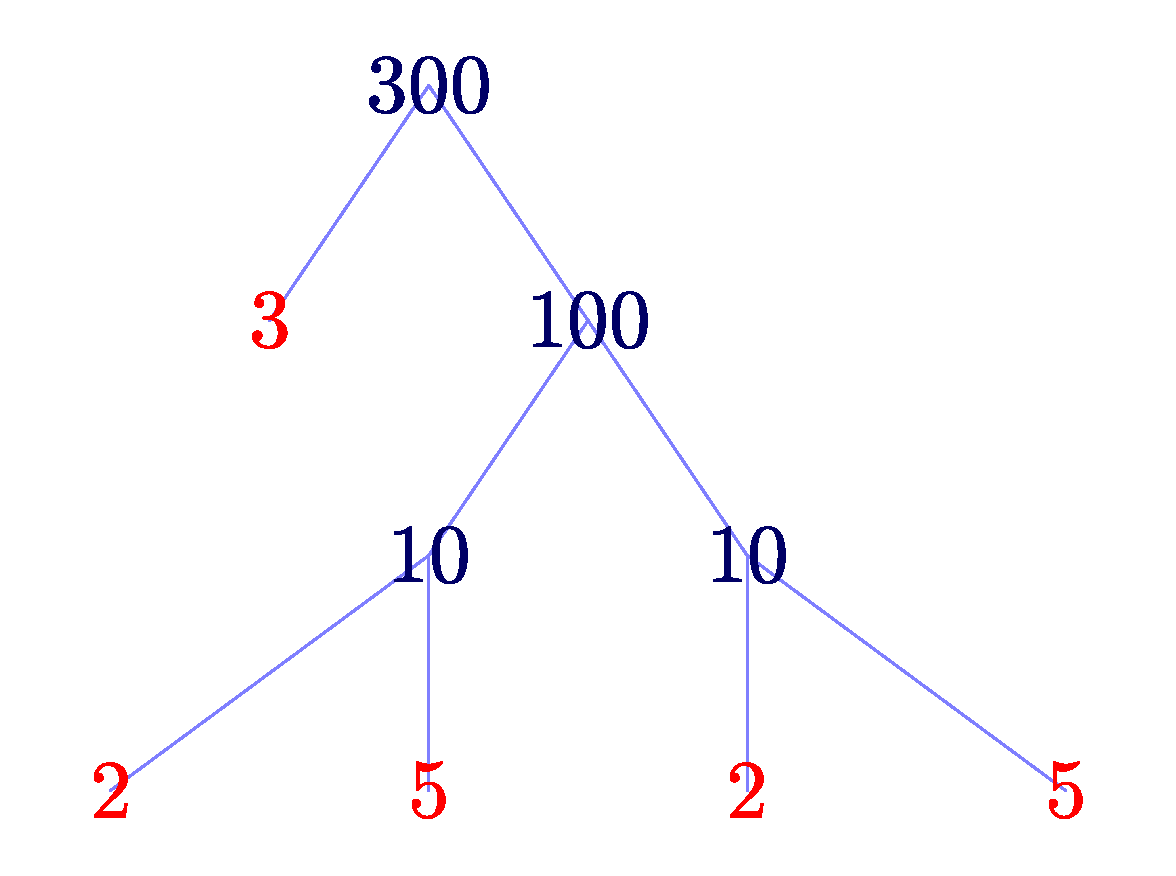
\includegraphics[width=0.47\textwidth]{illustrations/factor_tree_300_a}
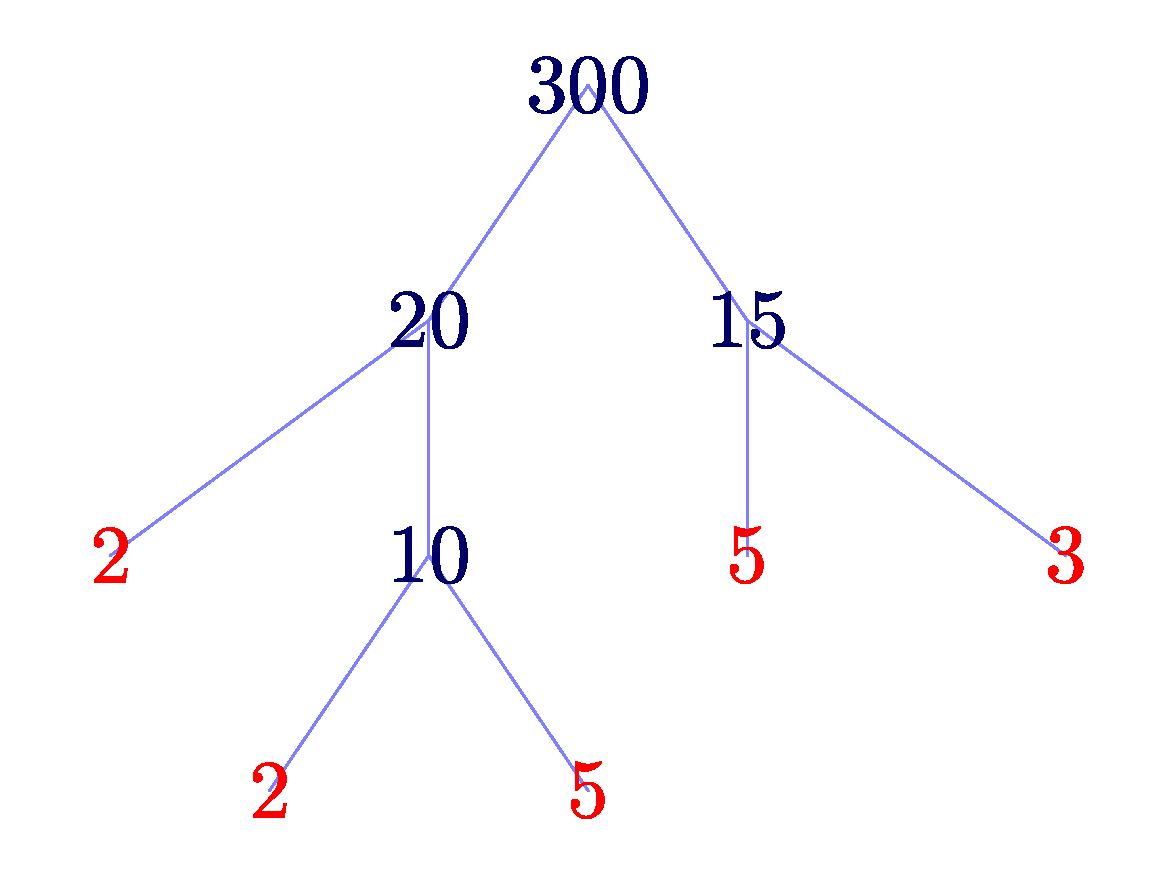
\includegraphics[width=0.47\textwidth]{illustrations/factor_tree_300_b}
\caption{Factor trees that illustrates the factorization of 300 as a product of primes.\label{fig:factor300}}
\end{center}
\end{figure}

\ill{factor_tree_big}{1}{Factorization tree for $6469693230$\label{factor.tree.big}}
 
                        
The Riemann Hypothesis probes the question: how intimately can we know
prime numbers, those {\em atoms} of multiplication?  Prime numbers are
an important part of our daily lives.  For example, anytime we visit a
website and purchase something online, prime numbers having over 150
decimal digits are used to keep our bank transactions private.  This
ubiquitous use to which these giant primes are put depends upon a very
simple principle: it is much easier to multiply numbers together than
to factor them. If you had to factor, say, the number $143$ you might
scratch your head for a few minutes before discovering that $143$ is
$11\times 13$. But if you had to multiply $11$ by $13$ you would do it
straightaway.  Offer two primes, say, $P$ and $Q$ each with more than
100 digits, to your computing machine and ask it to multiply them
together: you will get their product $N = P\times Q$ with its 200 or
so digits in a few microseconds. But present that number $N$ to any
current desktop computer, and ask it to factor $N$, and the computer
will (almost certainly) fail to do the task. The safety of much
encryption depends upon this guaranteed\endnote{Nobody has ever
  published a {\em proof} that there is no fast way to factor
  integers.  This is an article of ``faith'' among some
  cryptographers.} failure!

If we were latter-day number-phenomenologists we might revel in the
discovery and proof that
$$
  p=2^{43,112,609}-1
$$ 
is a prime number, this number having $12,\!978,\!189$ digits!  This
prime, which was discovered on August 23, 2008, was the first prime
ever found with more than ten million digits, whose discover won a
\$100,000 prize for the GIMPS project (\url{http://www.mersenne.org/}).

Now $2^{43,112,609}-1$ is quite a hefty number! Suppose someone came
up to you saying ``surely $p = 2^{43,112,609}-1$ is the largest prime
number!'' (which it is not) how might you convince that person that
he or she is wrong?

Here is a neat---and, we hope, convincing---strategy to show there are
prime numbers even larger than $p = 2^{43,112,609} - 1$. Imagine
forming the following humungous number: let $M$ be the product of all
prime numbers up to and including $p = 2^{43,11,2609} - 1$.  Now go
one further than $M$ by taking the next number $N=M+1$.
 

OK, even though this number $N$ is wildly large, it is either a prime
number itself---which would mean that there would indeed be a prime
number larger than $p=2^{43,112,609} - 1$, namely $N$; or in any event it is
surely divisible by some prime number, call it $P$.

Here, now, is a way of seeing that this $P$ is bigger than $p$: Since
every prime number smaller than or equal to $p$ divides $M$, these
prime numbers cannot divide $N= M+1$ (since they divide $M$ evenly, if
you tried to divide $N=M+1$ by any of them you would get a remainder
of $1$).  So, since $P$ does divide $N$ it must not be any of the
smaller prime numbers: $P$ is therefore a prime number bigger than $p=
2^{43,112,609}-1$.

You can think of this strategy as a simple game that you can
play. Start with any finite bag of prime numbers (say the bag that
only contains one prime, the prime $2$). Now each ``move'' of the game
consists of multiplying together all the primes you have in your bag
to get a number $M$, then adding $1$ to $M$ to get the even larger
number $N=M+1$, then factoring $N$ into prime number factors, and then
including all those new prime numbers in your bag. Euclid's proof
gives us that we will---with each move of this game---be finding more
prime numbers: the bag will increase. After, say, a million moves our
bag will be guaranteed to contain more than a million prime numbers.

For example, starting the game with your bag containing
only one prime number $2$, here is how your bag grows with after
successive moves of the game:

$\mbox{}\qquad\{2\}$
\newline
$\mbox{}\qquad\{2,3\}$
\newline
$\mbox{}\qquad\{2,3, 7\}$
\newline
$\mbox{}\qquad\{2,3, 7, 43\}$
\newline
$\mbox{}\qquad\{2,3, 7, 43, 13, 139\}$
\newline
$\mbox{}\qquad\{2,3, 7, 43, 13, 139, 3263443\}$
\newline
$\mbox{}\qquad\{2,3, 7, 43, 13, 139, 3263443,  547, 607, 1033, 31051\}$
\newline
$\mbox{}\qquad\{2,3, 7, 43, 13, 139, 3263443,  547, 607, 1033, 31051, 29881, 67003,
9119521, 6212157481\}$
\newline
\mbox{}\qquad{}etc.\endnote{The sequence of prime numbers we find by this
procedure is discussed in more detail with references at
Sloane's table of integer sequences:
\url{http://www.research.att.com/~njas/sequences/A126263}.}

This strategy, by the way, is not very new: it is, in fact, well over
two thousand years old, since it already occurred in Euclid's {\em
  Elements}. The Greeks did know that there are infinitely many prime
numbers and they showed it via the same method as we showed that our
$p = 2^{43,112,609} - 1$ is not the largest prime number.

Here is the argument again, given very succinctly: Suppose there are
only finitely many primes $p_1, \ldots, p_n$.  Let $n=p_1 p_2 \cdots
p_n + 1$.  Then $n$ is divisible by some prime, but no $p_i$ divides
$n$, which is contrary to our assumption that $p_1, \ldots, p_n$ is
the complete list of primes.

Though there are infinitely many primes, actually finding them is a
major challenge.  In the 1990s, the Electronic Frontier Foundation
\url{http://www.eff.org/awards/coop} offered a \$100,000 cash reward
to the first group to find a prime with at least 10,000,000 decimal
digits (the record prime $p$ above will win this prize), and offers
another \$150,000 cash prize to the first group to find a prime with
at least 100,000,000 decimal digits.

[[We could remark that there are infinitely many primes, but it
is {\em not} known whether or not there are infinitely
many Mersenne primes, i.e., primes of the form $2^p - 1$. ]]

The number $p$ displayed above is the largest prime we know, where by
``know'' we mean that we know it so explicitly that we can {\em
  compute} things about it.  For example, the last two digits of $p$
are 11 and the sum of the digits is 58,416,637.  Of course $p$ is not
the largest prime number since there are infinitely many primes, e.g.,
the next prime $q$ after $p$ is a prime.  But there is no obvious way
to efficiently compute anything interesting about $q$.  For example,
what is the last digit of $q$ in its decimal expansion?

\bigskip

%\ill{sieve_boxes_100}{0.7}{Sieve of Eratosthenes\label{fig:erat}}

Eratosthenes, the mathematician from Cyrene (and later, librarian at
Alexandria) explained how to {\em sift} the prime numbers from the
series of all numbers: in the sequence of numbers,
$$2\ \ 3\ \ 4 \ \ 5\ \ 6\ \ 7\ \ 8\ \ 9\ \ 10\ \ 11
\ \ 12\ \ 13\ \ 14\ \ 15\ \ 16\ \ 17\ \ 18\ \ 19\ \ 20\ \ 21\ \ 22\ \ 23\ \ 24\ \ 25\ \ 26\ \ 
27\ \ 28\ \ 29,$$
for example, start by circling the $2$ and crossing out all the other
multiples of $2$.  Next, go back to the beginning of our sequence of
numbers and circle the first number that is neither circled nor
crossed out (that would be, of course, the $3$), then cross out all
the other multiples of $3$.  This gives the pattern: go back again to
the beginning of our sequence of numbers and circle the first number
that is neither circled nor crossed out; then cross out all of its
other multiples.  Repeat this pattern until all the numbers in our
sequence are either circled, or crossed out, the circled ones being
the primes.



In Figure~\ref{fig:erat} we use the primes $2$, $3$, $5$, and $7$ to
sieve out the primes up to 100, where instead of crossing out
multiples we grey them out, and instead of circling primes we color
their box red.

\begin{figure}[H]
\begin{center}
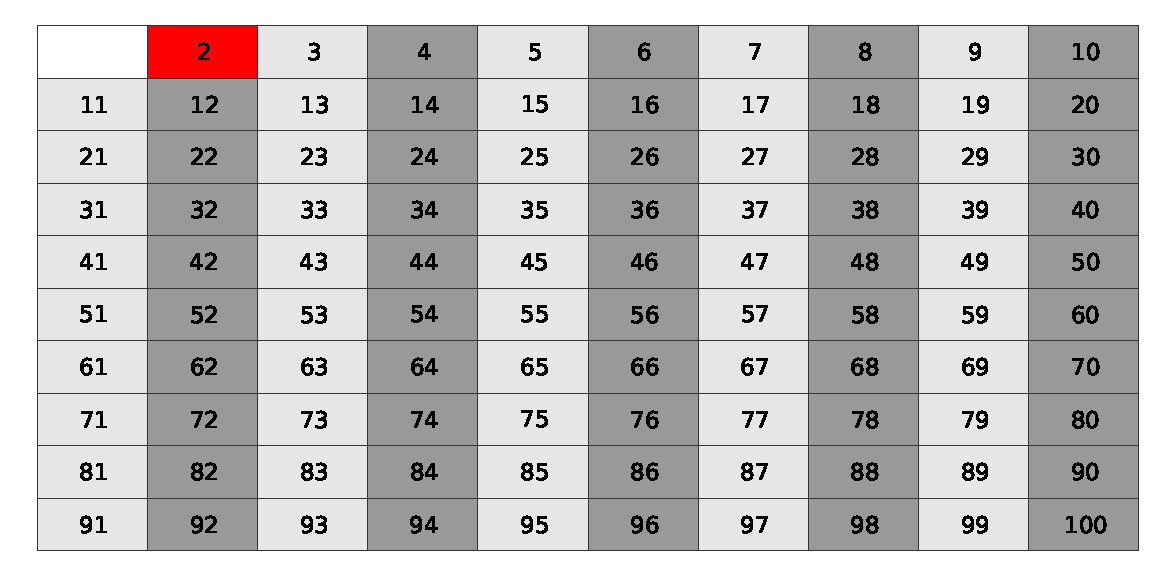
\includegraphics[width=.4\textwidth]{illustrations/sieve100-2}
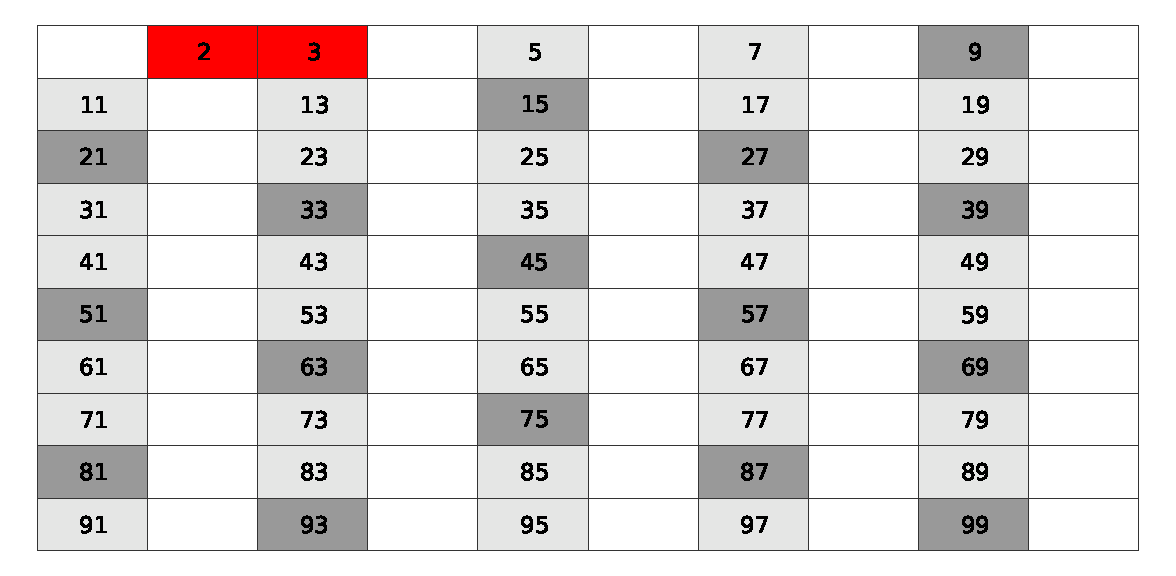
\includegraphics[width=.4\textwidth]{illustrations/sieve100-3}\\
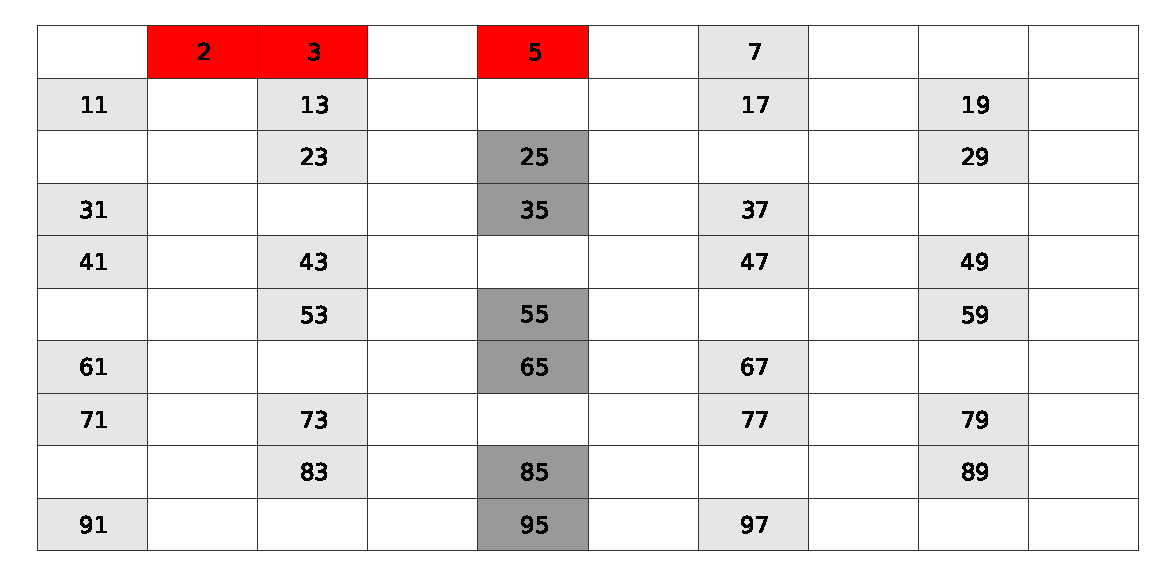
\includegraphics[width=.4\textwidth]{illustrations/sieve100-5}
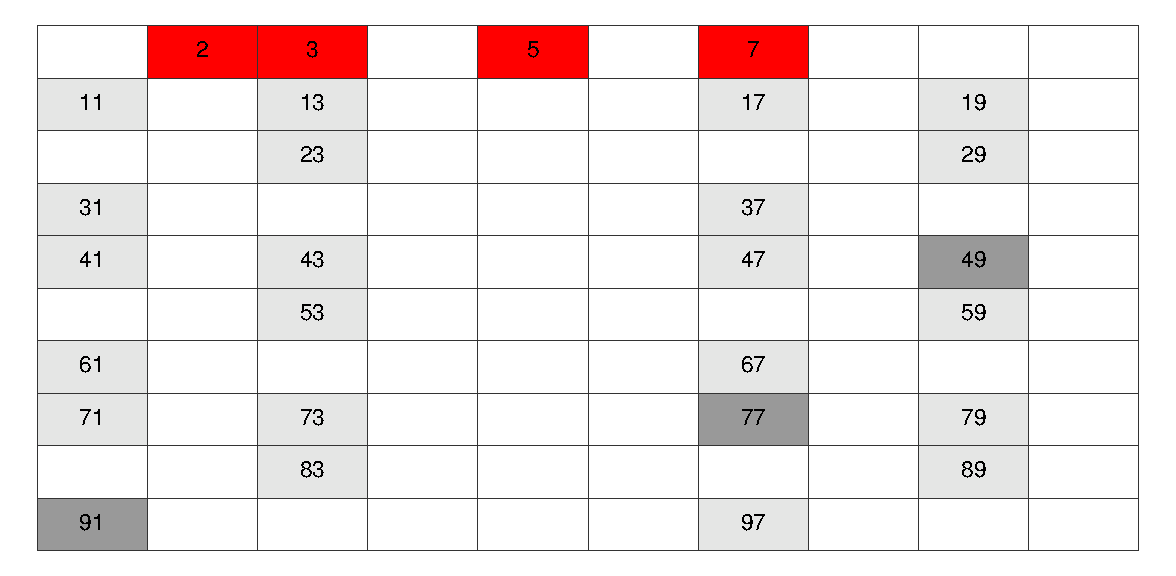
\includegraphics[width=.4\textwidth]{illustrations/sieve100-7}\\
\caption{Using the Primes 2,3,5,7 to Sieve out the Primes up to 100\label{fig:erat}}
\end{center}
\end{figure}


% GIVEN WHAT IS ABOVE, THIS IS SILLY.
%Especially if you have had little experience with math, may I suggest
%that you actually follow Eratosthenes' lead, and perform the repeated
%circling and crossing-out to watch the primes up to 100 emerge, intriguingly
%staggered through our sequence of numbers,
%$$2\ \ 3\ \ \bullet \ \ 5\ \ \bullet\ \ 7\ \ \bullet\ \ \bullet\ \ \bullet\ \ 11
%\ \ \bullet\ \ 13\ \ \bullet\ \ \bullet\ \ \bullet\ \ 17\ \ \bullet\ \ 19\ \ \bullet\ \ \bullet\ \
%\bullet\
%\ 23\ \ \bullet\ \ \bullet\ \ \bullet\ \  \bullet\ \ \bullet\ 29,\dots $$ 
%\bigskip

%\bigskip


\section{Questions about primes that any person might ask}

We become quickly stymied when we ask quite elementary questions about
the spacing of the infinite series of prime numbers.

\bigskip

For example, {\em are there infinitely many pairs of primes whose
  difference is $2$?}  The sequence of primes seems to be rich in such
pairs $$5-3 =2,\ \ \ 7-5=2,\ \ \ 13-11=2,\ \ \ 19-17 =2,$$ and we know
that there are loads more such pairs\endnote{For example, according to
\url{http://www.research.att.com/~njas/sequences/A007508} there are
$10,\!304,\!185,\!697,\!298$ such pairs less than
$10,\!000,\!000,\!000,\!000,\!000$.} but the answer to our question,
{\em are there infinitely many?}, is not known. {\em Are there
  infinitely many pairs of primes whose difference is $4$?}  Answer:
equally unknown. {\em Is every even number greater than $2$ a sum of
  two primes?}  Answer: unknown. {\em Are there infinitely many primes
  which are $1$ more than a perfect square?}  Answer: unknown.


\bigskip

Remember the Mersenne prime $p= 2^{43,112,609}-1$? and how we showed
that there is a prime $P$ larger than that? Suppose, though, someone
asked us whether there was a {\it Mersenne Prime} larger than this
$p$: that is, {\em is there a prime number of the form $$2^{\rm some\
  prime\ number}-1$$ bigger than $p= 2^{43,112,609}-1$?} Answer:  We don't
know. It is possible that there are infinitely many Mersenne primes
but we're far from being able to answer such questions.

\bigskip


{\em Is there some neat formula giving the next prime?} More
specifically, {\em If I give you a number $N$, say $N=$ one million,
  and ask you for the first number after $N$ that is prime, is there a
  method that answers that question without, in some form or other,
  running through each of the successive odd numbers after $N$ rejecting
  the nonprimes until the first prime is encountered?}  Answer:
unknown.

\bigskip
%%%%%%%%%%%%%%%

One can think of many ways of ``getting at'' some understanding of the
placement of prime numbers among all number.  Up to this point we have
been mainly just counting them, trying to answer the question ``how
many primes are there up to $X$?''  and we have begun to get some feel
for the numbers behind this question, and especially for the current
``best guesses'' about estimates.
   

What is wonderful about this subject is that people attracted to it
cannot resist asking questions that lead to interesting, and sometimes
surprising numerical experiments. Moreover, given our current state of
knowledge, many of the questions that come to mind are still
unapproachable: we don't yet know enough about numbers to answer them.
But {\it asking interesting questions} about the mathematics that you
are studying is a high art, and is probably a necessary skill to
acquire, in order to get the most enjoyment---and understanding---from
mathematics.  So, we offer this challenge to you:

Come up with with your own question about primes that:
 
 \begin{itemize}
 \item     is interesting to you,
  \item    is not a question whose answer is known to you,
 \item     is not a question that you've seen before; or at least not exactly,
  \item    is a question about which you can begin to make numerical investigations? 
 \end{itemize}
 
\subsection{Further questions about primes} 

Let us, for variety, dice the question differently by concentrating on
the {\em gaps} between one prime and the next, rather than the tally
of all primes. Of course, it is no fun at all to try to guess how many
pairs of primes $p, q$ there are with gap $q-p$ equal to to a fixed
odd number.  The fun, though, begins in earnest if you ask for pairs
of primes with difference equal to $2$ (these being called {\em twin
  primes}) for it has long been guessed that there are infinitely many
such pairs of primes, but no one has been able to prove this yet.

\begin{quote} The largest known twin primes are 
$$65516468355\cdot 2^{333333} \pm 1$$
They have $100355$ digits and were announced by Kaiser and Klahnin
$2009$.
\end{quote}


Similarly with difference $4$, or $8$, or---in fact---any even number
$2k$. That is, people have guessed that there are infinitely many
pairs of primes with difference $4$, with difference $6$, etc. but
none of these guesses have yet been proved. [[maybe reference in an
endnote something involving Green/Tao or Goldstein or some other
recent big theorem related to the above?]]




   
So, define $${\rm Gap}_{k}(X)$$ to be the number of pairs of primes
less than $X$ with ``gap $k$'' (i.e., such that their difference is
$k$).  For example, ${\rm Gap}_2(10) = 2$, since the pairs $(3,5)$ and
$(5,7)$ are the pairs less than $10$ with gap $2$.
See Table~\ref{tab:gap} for various values of ${\rm Gap}_{k}(X)$.
   
   \bigskip
   
\begin{figure}[H]
\begin{center}
\caption{Values of ${\rm Gap}_{k}(X)$ \label{tab:gap}}
\vspace{1em}

\begin{tabular}{|l|c|c|c|c|}\hline
$X$ & ${\rm Gap}_{2}(X)$ & ${\rm Gap}_{4}(X)$& ${\rm Gap}_{6}(X)$ & ${\rm Gap}_{8}(X)$\\\hline
10 & 2 & 1 & 0 & 0\\\hline
$10^2$ & 8 & 8 & 7 & 1 \\\hline
$10^3$ & 35 & 40 & 44 & 15 \\\hline
$10^4$ & 205 & 202 & 299 & 101 \\\hline
$10^5$ & 1224 & 1215 & 1940 & 773 \\\hline
$10^6$ & 8169 & 8143 & 13549 & 5569 \\\hline
$10^7$ & 58980 & 58621 & 99987 & 42352 \\\hline
\end{tabular}
\end{center}
\end{figure}   

   \bigskip
   
   Here is yet another question with deals with
the spacing of prime numbers that we can't answer.
  
{\em Racing Gap $2$,  Gap $4$, Gap $6$, and Gap $8$ against each other:} 
  
\begin{quote}
  Challenge: As X tends to infinity which of the three $Gap_2(X),
  Gap_4(X), Gap_6(X),$ or $Gap_8(X)$ do you think that will grow
  faster? How much would you bet on the truth of your guess?
\end{quote}
  
[[TODO: It would be natural to talk about the
conjectural Hardy-Littlewood answer to this question, which is very
much not suggested by data.  Perhaps we should also
ask whether ${\rm Gap}_6(X)$ is always the winner, or if there is some
other $k$ such that ${\rm Gap}_k(X)$ eventually always beat ${\rm
  Gap}_6(X)$?  That's what Hardy-Littlewood predicts.]]

[[Give Hardy-Littlewood's asymptotic conjecture for $Gap_k(X)$ (I
assume it is simply $C_k{\sqrt X}/\log(X)$ for some specific
(nonzero...)  constants $C_k$? What are these $C_k$'s???  Should we
just trot them out in a little table, and say that this is Hardy and
Littlewood's guess, but we haven't a clue, at present, how to prove
such guesses.]]


Here is a curious question that you can easily begin to check out for
small numbers. We know, of course, that the {\em even} numbers and the
{\em odd} numbers are nicely and simply distributed: after every odd
number comes an even number, after every even, an odd, there is an
equal number of odd number as even numbers less than any given odd
number, and there may be nothing else of interest to say about the
matter.  Things change considerably, though, if we focus our
concentration on {\em multiplicatively even} numbers and {\em
  multiplicatively odd} numbers.
  
  
A {\bf multiplicatively even} number is one that can be expressed as a
product of {\em an even number of} primes; and a {\bf multiplicatively
  odd} number is one that can be expressed as a product of {\em an odd
  number of} primes.  So, any prime is multiplicatively odd, the
number $4 = 2\cdot 2$ is multiplicatively even, and so is $6=2\cdot
3$, $9=3\cdot 3$, and $10= 2\cdot 5$; but $12=2\cdot 2\cdot 4$ is
multiplicatively odd.  Here is some data: \newpage
   
  \begin{table} \caption{Multiplicatively even and odd positive numbers $\le N$}
  \begin{center}
 
\begin{tabular}{|l|r|r|r|r|r|r|r|r|r|r|r|r|r|r|r|}
\hline
N & 2 & 3 & 4 & 5  & 6 & 7 & 8 & 9 & 10 & 11 & 12 & 13 & 14 & 15 & 16  \\ \hline
Multiplicatively even & 1 & 1 & 2 & 2  & 3 & 3 & 3 & 4 & 5 & 5 & 5 & 5 & 6 & 7 & 8 \\ \hline
Multiplicatively odd & 1 & 2 & 2 & 3  & 3 & 4 & 5 & 5 & 5 & 6 & 7 & 8 & 8 & 8 & 8 \\ \hline
\end{tabular}
\end{center}
\end{table}

  
   Now looking at this data, a natural, and simple, question to ask about the concept of multiplicative {\em oddness} and {\em evenness} is: 
   
   \noindent {\em Is there some  $N\ge 2$ for which there are more multiplicatively even numbers less than or equal to $N$ than multiplicatively odd ones?}

Each plot in Figure~\ref{fig:liouville} gives the number of
multiplicatively even numbers between $2$ and $N$ minus the number of
multiplicatively odd numbers between $2$ and $N$, for $N$ equal to 10,
100, 1000, and 10000. The above question asks whether these graphs
would, for sufficiently large $N$, ever cross the $x$-axis.

 \begin{figure}[H]
\begin{center}
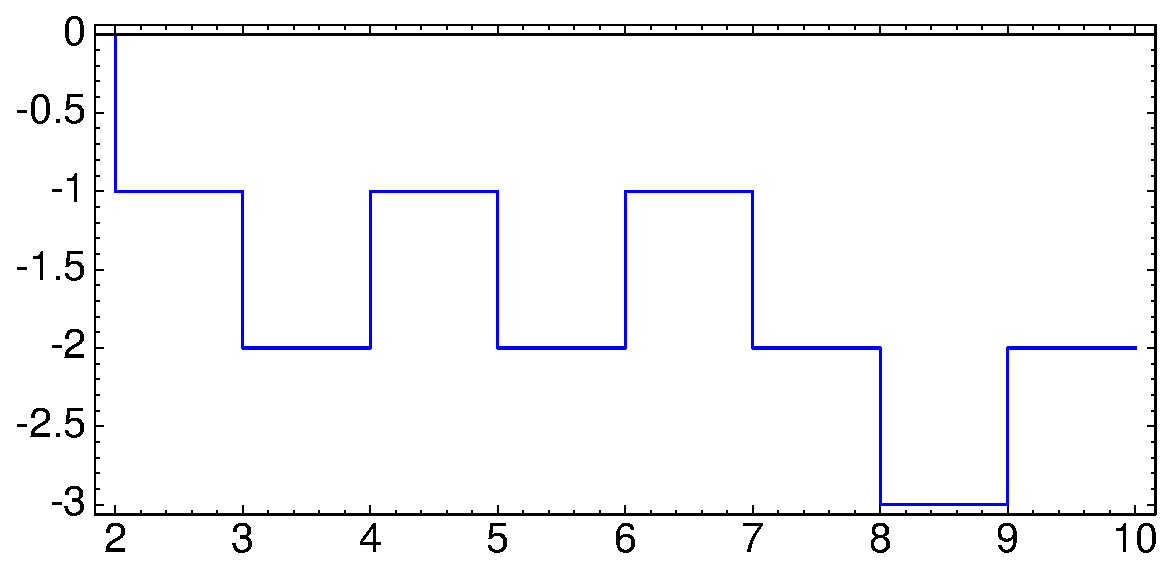
\includegraphics[width=.4\textwidth]{illustrations/liouville-10}
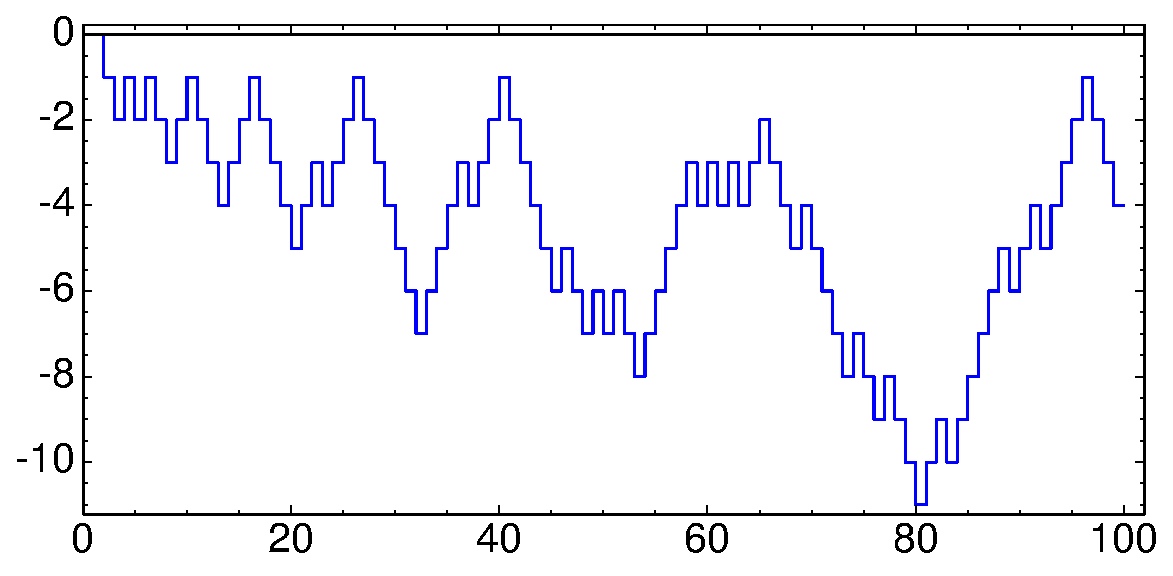
\includegraphics[width=.4\textwidth]{illustrations/liouville-100}\\
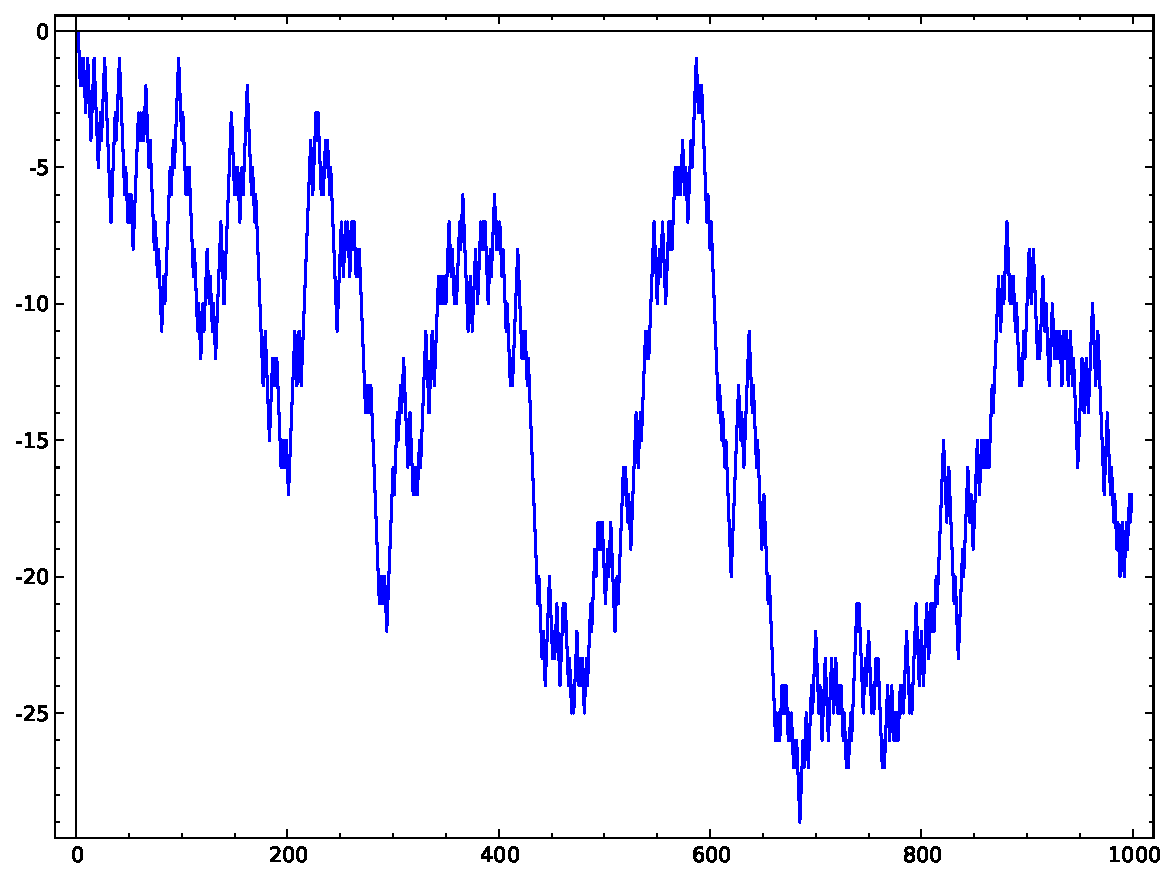
\includegraphics[width=.4\textwidth]{illustrations/liouville-1000}
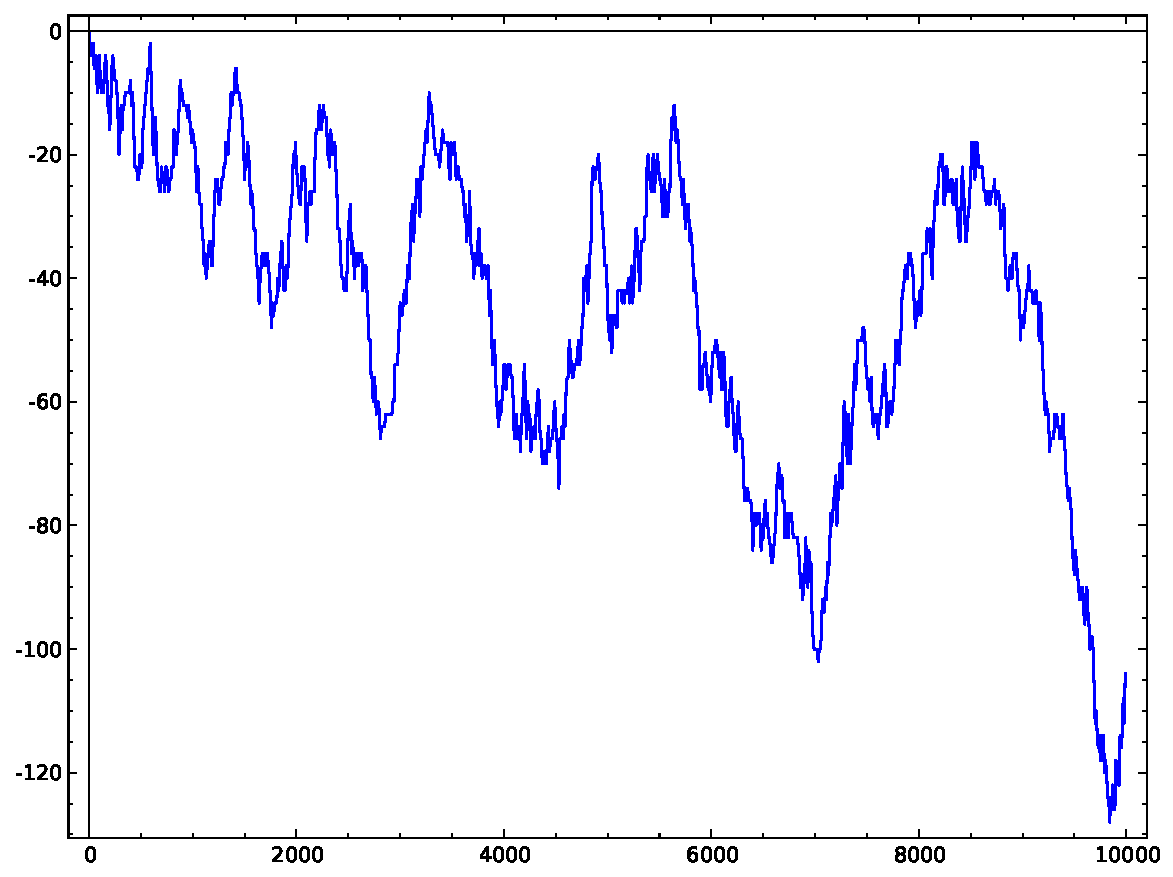
\includegraphics[width=.4\textwidth]{illustrations/liouville-10000}\\
\caption{Racing Multiplicatively Even and Odd Numbers\label{fig:liouville}}
\end{center}
\end{figure}
  
A {\em negative} response to this question would imply the Riemann
Hypothesis!  In contrast to the list of previous questions, the answer
to this one is known: alas, there is such an $N$.  In 1960, Lehman
showed that for $N=906,400,000$ there are $708$ more multiplicatively
even numbers up to $N$ than multiplicatively odd numbers (Tanaka found
in 1980 that the smallest $N$ with this property is
$N=906,150,257$). For more details, see P.~Borwein, {\em Sign changes
  in sums of the Liouville Function} and the nice short paper of
Norbert Wiener {\em Notes on Polya's and Turan's hypothesis concerning
  Liouville's factor} (page 765 of volume II of Wiener's Collected
Works); see also: G. Polya {\em Vershiedene Bemerkungen zur
  Zahlentheorie} Jahresbericht de Deutschen Mathematiker-Vereinigung,
{\bf 28} (1919) 31--40.

%%%%%%%%%%%%%%%%%

These are questions that have been asked about primes (and we could
give bushels more), questions expressible in simple vocabulary, that
we can't answer today. We have been studying numbers for over two
millenia and yet we are indeed in the infancy of our understanding.

So we'll continue our discussion by returning to the simplest counting
question about prime numbers.

                           
\section{How many primes are there?}

\ill{sieve200}{.7}{Sieving Primes up to 200}
                                                      
Slow as we are to understand primes, at the very least we can try to
count them. You can see that there are $10$ primes less than $30$, so
you might encapsulate this by saying that the chances that a number
less than $30$ is prime is $1$ in $3$.  This frequency does not
persist, though; here is some more data: There are $25$ primes less
than $100$ (so $1$ in $4$ numbers up to $100$ are prime), there are
$168$ primes less than a thousand (so we might say that among the
numbers less than a thousand the chances that one of them is prime is
roughly $1$ in $6$).
                                                           
\ill{proportion_primes_100}{0.9}{Proportion of primes up to $N=100$}

There are 78,498 primes less than a million (so we might say that
the chances that a random choice among the first million numbers is
prime have dropped to roughly $1$ in $13$).

\illtwo{proportion_primes_1000}{proportion_primes_10000}{0.4}{Proportion of primes up to $1000$ and $10000$}

There are 455,052,512 primes less than ten billion; i.e.,
10,000,000,000 (so we might say that the chances are down to roughly
$1$ in $22$).

Primes, then, seem to be thinning out.  We return to the sifting process
we did earlier, and take a look at a few graphs, to get a sense of why
that might be so. There are a hundred numbers less than or equal to
$100$, a thousand numbers less than or equal to $1000$, etc.: the
shaded bar graph that looks like a regular staircase, each step the
same length as each riser, climbing up at, so to speak, a 45 degree
angle, counts all numbers up to and including $N$.

Following Eratosthenes, we have sifted those numbers, to pan for
primes. Our first move was to throw out roughly half the numbers (the
even ones!) after the number $2$. The cross-hatched bar graph in this
figure which is, with one hiccup, a regular staircase climbing at a
smaller angle, each step twice the lengths of each riser, illustrates
the numbers that are left after one pass through Eratosthenes' sieve,
which includes, of course, all the primes. So, the chances that a
number bigger than $2$ is prime is {\em at most} $1$ in $2$.  Our
second move was to throw out a good bunch of numbers bigger than $3$.
So, the chances that a number bigger than $3$ is prime is going to be
even less.  And so it goes: with each move in our
sieving process we are winnowing the field more extensively, reducing
the chances that the later numbers are prime.

\illtwo{sieve_2_200}{sieve1000}{.45}{Sieving by removing multiples of $2$ up to $100$ and Sieving for primes up to $1000$}
          
The red curve in these figures actually counts the primes: it is the
beguilingly irregular {\em staircase of primes.}  Its height above any
number $N$ on the horizontal line records the number of primes less
than or equal to $N$, the accumulation of primes up to $N$.  Refer to
this number as $\pi(X)$. So $\pi(2)=1$, $\pi(3) = 2$, $\pi(30) = 10$; of
course, if you believed some of the data above you could plot a few
more values of $\pi(X)$, like $\pi(\text{ten billion}) = 455,052,512$.
                              
                                 
Let us accompany Eratosthenes for a few further steps in his sieving
process.  Figure~\ref{fig:sieve3_100} contains a graph of all whole
numbers up to 100 after we have removed the even numbers greater than
$2$, and the multiples of $3$ greater than $3$ itself.
                                 
\begin{figure}[H]
\begin{center}
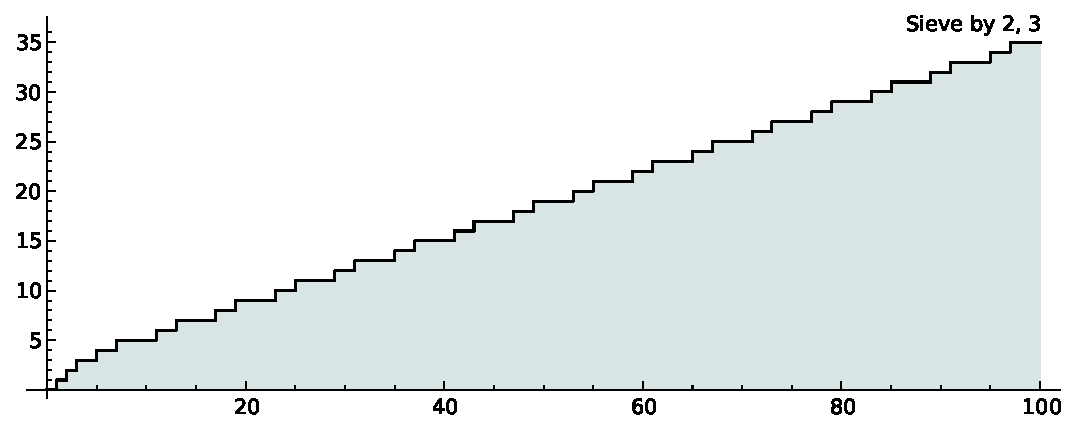
\includegraphics[width=0.5\textwidth]{illustrations/sieves3_100}
\caption{Sieving out multiples of $2$ and $3$.\label{fig:sieve3_100}}
\end{center}
\end{figure}

From this graph you can see that if you go ``out a way'' the
likelihood that a number is a prime is less that $1$ in $3
$. Figure~\ref{fig:sieve7_100} contains a graph of what Eratosthenes
sieve looks like up to 100 after sifting $2,3,5,$ and $7$.


\begin{figure}[H]
\begin{center}
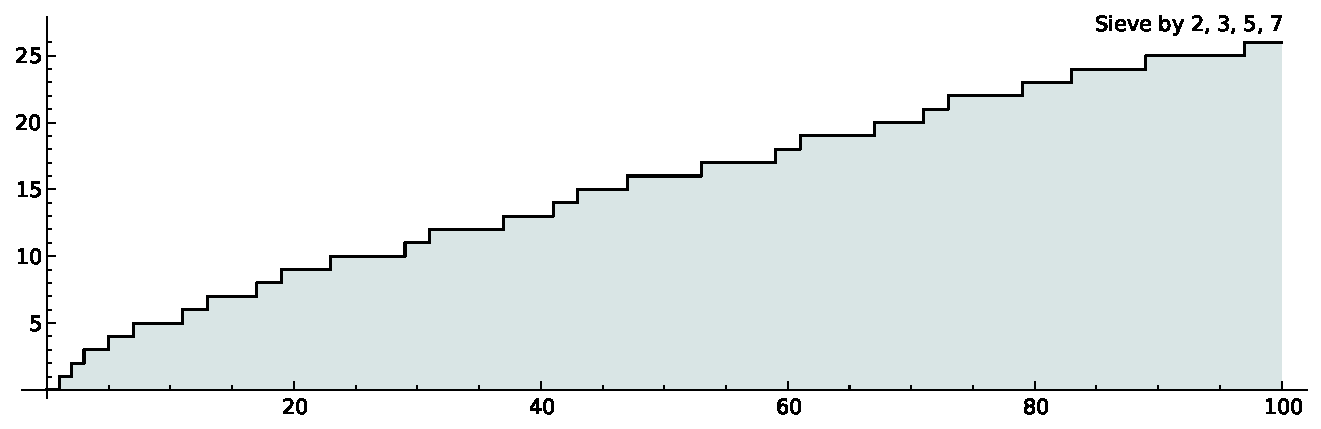
\includegraphics[width=0.5\textwidth]{illustrations/sieves7_100}
\caption{Sieving out multiples of $2$, $3$, $5$, and $7$.\label{fig:sieve7_100}}
\end{center}
\end{figure}


This data may begin to suggest to you that as you go further and
further out on the number line the percentage of prime numbers among
all whole numbers tends towards $0\%$ (it does).
  

To get a sense of how the primes accumulate, we will take a look at
the staircase of primes for $N= 25$, and $N=100$.


\illtwo{PN_25}{PN_100}{.33}{}

    
    
\section{Prime numbers viewed from a distance}
The striking thing about these figures is that as the numbers get
large enough, the jagged accumulation of primes, those
quintessentially discrete entities, becomes smoother and smoother, to
the eye. How strange and wonderful to watch, as our viewpoint zooms
out to larger ranges of numbers, the accumulation of primes taking on
such a smooth and elegant shape.

\illtwo{PN_1000}{PN_10000}{.33}{}

   \begin{figure}[H]
   \begin{center}
   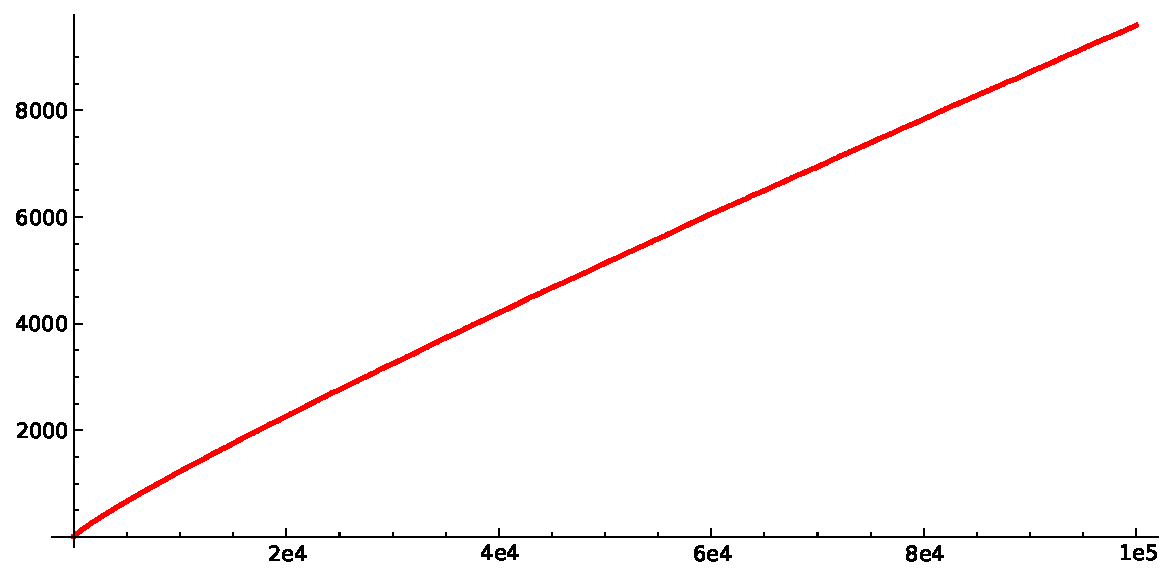
\includegraphics[width=.7\textwidth]{illustrations/PN_100000}
   \caption{Primes up to 100,000\label{fig:pn100000}}
   \end{center}
    \end{figure}

But don't be fooled by the seemingly smooth shape of the curve in the
last figure above: it is just as faithful a reproduction of the
staircase of primes as the typographer's art can render, for there are
thousands of tiny steps and risers in this curve, all hidden by the
thickness of the print of the drawn curve in the figure.  It is
already something of a miracle that we can approximately describe the
build-up of primes, somehow, using a {\em smooth curve}.  But {\em
  what} smooth curve?


That last question is {\em not} rhetorical. If I draw a curve with
chalk on the blackboard, this can signify a myriad of smooth
(mathematical) curves all encompassed within the thickness of the
chalk-line, all--if you wish--reasonable approximations of one
another. So, there are many smooth curves that fit the chalk-curve.
With this warning, but very much fortified by the data of Figure~\ref{fig:pn100000},
let us ask: {\em what is a smooth curve that is a reasonable
  approximation to the staircase of primes?}

\section{ Pure and applied  mathematics  }     

Everyone seems to agree that, loosely speaking, there are two types of
mathematics: {\em pure} and {\em applied}. Usually---when we judge
whether a piece of mathematics is pure or applied---this distinction
turns on whether or not the math has application to the ``outside
world,'' i.e., that {\em world} where bridges are built, where economic
models are fashioned, where computers churn away at the internet (for
only then do we unabashedly call it {\em applied math}), or whether
the piece of mathematics will find an important place within the
context of mathematical theory (and then we label it {\em pure}).  Of
course, there is a great overlap. Moreover, many questions in
mathematics are ``hustlers'' in the sense that, at first view, what is
being requested is that some simple task be done (e.g., the question
raised in this book, {\em to find a smooth curve that is a reasonable
  approximation to the staircase of primes}).  And only as things
develop is it discovered that there are payoffs in many unexpected
directions, some of these payoffs being genuinely applied (i.e., to
the practical world), some of these payoffs being pure (allowing us
to strike behind the mask of the mere appearance of the mathematical
situation, and get at the hidden fundamentals that actually govern the
phenomena), and some of these payoffs defying such simple
classification, insofar as they provide powerful techniques in other
branches of mathematics.  The Riemann Hypothesis---even in its current
unsolved state---has already shown itself to have all three types of
payoff.

The particular issue before us is, in our opinion, twofold, both
applied, and pure: can we curve-fit the ``staircase of primes'' by a
well approximating smooth curve?  The story behind this alone is
marvelous, has a cornucopia of applications, and we will be telling it
below. But our curiosity here is driven by a question that is pure,
and less amenable to precise formulation: are there mathematical
concepts at the root of, and more basic than (and ``prior to,'' to
borrow Aristotle's use of the phrase,) {\em prime numbers}--concepts
that account for the apparent complexity of the nature of primes?
   
   
%[[TODO (william): Insert a discussion here about how believing RH is
%crucial to doing many algebraic number theory calculations.  E.g.,
%complexity analyses for algorithms like factoring depend on RH.  Also,
%standard class group algorithms are vastly faster if we assume RH (or
%even more!), so number theorists do so all the time when doing
%numerical experiments (though of course they try to remove the
%hypothesis...).  See {\tt
%  http://pari.math.u-bordeaux.fr/dochtml/html.stable/}, e.g., for some
%sense of what this is like in the trenches...  It says ``Warning. Make
%sure you understand the above!'']]
   
\section{A probabilistic ``first'' guess }
The search for such approximating curves began, in fact, two centuries
ago when Carl Friedrich Gauss defined a certain beautiful curve that,
experimentally, seemed to be an exceptionally good fit for the
staircase of primes. Let us denote Gauss's curve $G(X)$; it has an
elegant simple formula comprehensible to anyone who has had a tiny bit
of calculus.  If you make believe that the chances that a number $N$ is
a prime is inversely proportional to the number of digits of $N$ you
might well hit upon Gauss's curve.   In a letter written in 1849, Gauss
claimed that as early as 1792 or 1793 he had already observed that the
density of prime numbers over intervals of numbers of a given rough
magnitude $X$ seemed to average $1/\log(X)$.  Roughly speaking, this
means that the number of primes up to $X$ is $X$ times the reciprocal 
of $2.3$ times the number of digits of $X$.  For example,
the number of primes less than $99$ should be roughly
$$
   {\frac{1}{2\times 2.3}}\times 99\ \approx \ 22,
$$   
which is pretty close, although an undercount: the correct number of
primes $< 99$ is $25$.  The number of primes up to $999$ should
be roughly
$$
   {\frac{1}{3\times 2.3}}\times 999\ \approx \ 145,
$$   
which is again close, since there are 168 primes up to below $100$. 
The number of primes up to $999,\!999$ should be roughly
$$
   {\frac{1}{6\times 2.3}}\times 999999\ \approx \ 72464,
$$   
which is close to the correct count of $78,\!498$.

\illthree{area_under_graph_30}{area_under_graph_100}{area_under_graph_1000}{.3}{The
  expected tally of the number of primes $<X$ is approximated by the
  area underneath the graph of $1/\log(X)$ from $1$ to $X$.}

           
Gauss was an inveterate computer: he wrote in his 1849 letter that
there are $216,\!745$ prime numbers less than three million (This is
wrong: the actual number of these primes is $216,\!816$). Gauss's curve
predicted that there would be $216,\!971$ primes-- a miss, Gauss
thought, by $226$ (but actually he was closer than he thought: the
correct {\em miss} is a mere $161$; not as close as the 2004 US
elections, but pretty close nevertheless).  
Gauss's computation brings up two queries: will this spectacular ``good
fit'' continue for arbitrarily large numbers? and, the (evidently
prior) question: what counts as a good fit?


\section{What is a ``good approximation''?}\label{sec:sqrterror}

If you are trying to estimate a number, say, around ten thousand, and
you get it right to within a hundred, let us celebrate this kind of
accuracy by saying that you have made an approximation with {\em
  square-root error} (${\sqrt{10,\!000}}=100$). Of course, we should
really use the more clumsy phrase ``an approximation with at worst
{\em square-root error.}''  Sometimes we'll simply refer to such
approximations as {\em good approximations.} If you are trying to
estimate a number in the millions, and you get it right to within a
thousand, let's agree that---again---you have made an approximation
with {\em square-root error} (${\sqrt{1,\!000,\!000}}=1,\!000$).
Again, for short, call this a {\em good approximation.} So, when Gauss
thought his curve missed by $226$ in estimating the number of primes
less than three million, it was well within the margin we have given
for a ``good approximation.''

More generally, if you are trying to estimate a number that has $D$
digits and you get it almost right, but with an error that has no more
than, roughly, half that many digits, let us say, again, that you have
made an approximation with {\em square-root error} or synomymously, a
{\em good approximation}.


This rough account almost suffices for what we will be discussing
below, but to be more precise, the specific {\em gauge of accuracy}
that will be important to us is not for a mere {\em single} estimate
of a {\em single} error term, \bigskip
 
 \centerline{Error term\ \  =\ \    Exact Value\ \   -\ \   Our ``good  approximation''}
  
 \bigskip
 
 \noindent but rather for {\em infinite sequences} of estimates of
 error terms. Generally, if you are interested in a numerical quantity
 $q(X)$ that depends on the real number parameter $X$ (e.g., $q(X)$
 could be $\pi(X)$, ``the number of primes $< X$'') and if you have an
 explicit candidate ``approximation,'' $q_{\rm approx}(X)$, to this
 quantity, let us say that $q_{\rm approx}(X)$ is {\bf essentially a
   square-root accurate approximation to $q(X)$} if for {\em any}
 given exponent greater than $0.5$ (you choose it: $0.501$, $0.5001$,
 $0.50001$, $\dots$ for example) and for large enough $X$--- where the
 phrase ``large enough'' depends on your choice of exponent---the {\bf
   error term}---i.e., the difference between $q_{\rm approx}(X)$ and
 the {\em true} quantity, $q(X)$, is, in absolute value, less than
 $q_{\rm approx}(X)$ raised to that exponent (e.g. $< X^{0.501}$, $<
 X^{0.5001}$, etc.). Readers who know calculus and wish to have a
 technical formulation of this definition of {\em good approximation}
 might turn to the endnote $^2$ for a precise statement.

\begin{remark}
  To get a feel for how basic the notion of {\em approximation to data
    being square root close to the true values of the data} is---and
  how it represents the ``gold standard'' of accuracy for
  approximations, consider this fable.


  Imagine that the devil had the idea of saddling a large committee of
  people with the task of finding values of $\pi(X)$ for various large
  numbers $N$.  This he did in the following somewhat ridiculous
  manner, having already worked out which numbers are prime and which
  composite, himself. Since the devil is, as everyone knows, {\em into
    the details,} he has made no mistakes: his work is entirely
  correct.  He gives each committee member a copy of the list of all
  whole numbers between $1$ and one of the large numbers $N$ in which
  he was interested, the devil having put check-marks by the numbers
  on that list that are prime numbers, and no mark by the composite
  numbers. Now each committee member would count the number of primes
  by considering each number, in turn, on their list to figure out
  whether or not there is a check beside it, and tally up the ones
  that have checks. But since they are human, they will indeed be
  making mistakes, say $0.001\%$ of the time.  Assume further that it
  is just as likely for them to make the mistake of thinking that a
  number {\em has} a check-mark that does not have one, as the
  contrary: that a number hasn't got a mark, when it does.  If many
  people are engaged in such pursuit, some of them might over-count
  $\pi(X)$; some of them might under-count it. The average error
  (over-counted or undercounted) would be proportional to~${\sqrt N}$.

\end{remark}

\section { What is Riemann's Hypothesis?  ({\em first formulation})\label{sec:rh1}}

\bigskip 

Recall that a rough approximation to $\pi(X)$, the number of primes $<
X$,  is given by the function $X/\log(X)$; and  Gauss's guess for an
approximation to $\pi(X)$  was in terms of the area in the region
from $2$ to $X$ under the graph $1/\log(X)$, a quantity sometimes referred to
as $\Li(X) = \int_2^X (dx/\log x)$.
``Li'' (pronounced L$\overline{\rm i}$) is short for {\em logarithmic integral}.


Figure~\ref{fig:threeplots} contains a graph of the three functions
$\Li(X)$, $\pi(X)$, and $X/\log X$ for $X\leq 200$.
 
\begin{figure}[H]
\begin{center}
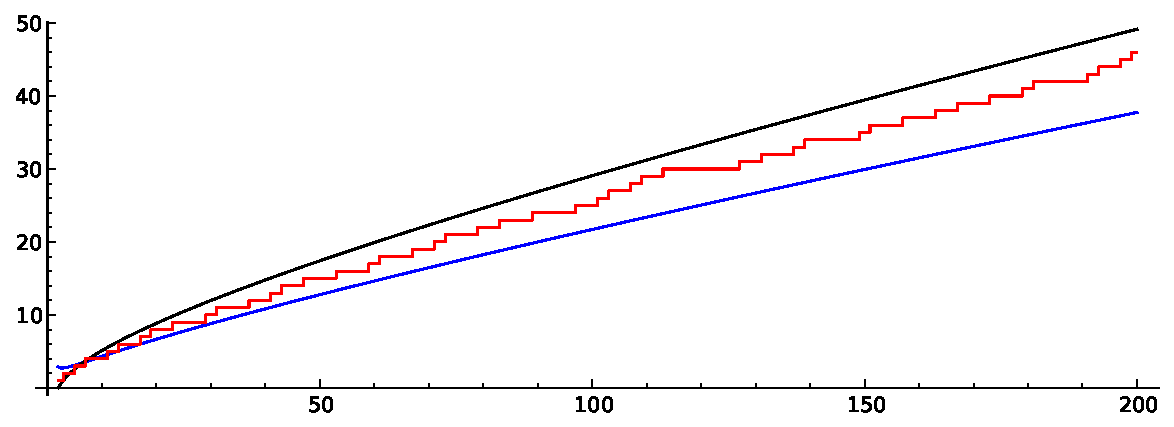
\includegraphics[width=.7\textwidth]{illustrations/three_plots}
\caption{Plots of $\Li(X)$ (top), $\pi(X)$ (in the middle), and $X/\log(X)$ (bottom)\label{fig:threeplots}}
\end{center}
\end{figure}
 
Let $X=4\cdot 10^{22}$.  Then \label{pili_vals}
\begin{align*}
  \pi(X) &= 783964159847056303858,\\
  \Li(X) &= 783964159852157952242.7155276025801473\ldots, \\
  X/(\log(X)-1)  &=  783650443647303761503.5237113087392967\ldots.\\
  |\pi(X) - \Li(X)| &= 5101648384.71552760258014\ldots, \\
  \sqrt{X}\log(X) &=  10408633281397.77913344605\ldots,
\end{align*}
The computation of $\pi(X)$ above is a major distributed computation
that is described at \url{http://numbers.computation.free.fr/Constants/Primes/Pix/pixproject.html}.

 

Since $\Li(X)$ seems to start out impressively close in value to our
$\pi(X)$ (at least in this range) it is natural to hope that in full
generality it is {\it essentially a square root approximation} to
$\pi(X)$.  This gives us our first formulation of Riemann's
Hypothesis:

      \begin{center}
       \shadowbox{ \begin{minipage}{0.9\textwidth}
\mbox{}       \vspace{0.2ex}
       \begin{center}{\bf\large The {\bf Riemann Hypothesis} (first formulation)}\end{center}
       \medskip

For any real number $X$ the number of prime numbers less than $X$ is
approximately $\Li(X)$ and this approximation is essentially square
root accurate.

\vspace{1ex}
\end{minipage}}
      \end{center}
 
\bigskip
 


\section{The Prime Number Theorem}
  
Take a look at Figure 10.1 again.  All three functions, $X/\log(X)$,
$\Li(X)$ and $\pi(X)$ are ``going to infinity with $X$'' (this means
that for any real number $R$, if $X$ is taken to be sufficiently
large, the values of these functions at $X$ will exceed $R$).

Are these functions ``going to infinity'' at {\it the same rate}?

To answer such a question, we have to know what we mean by {\it going
  to infinity at the same rate}. So, here's a definition. Two
functions, $A(X)$ and $B(X)$, that each go to infinity will be said to
{\bf go to infinity at the same rate} if their {\it ratio}
$$A(X)/B(X)$$ 
tends to $1$ as $X$ goes to infinity.


[[insert example plot??]]

For example, two polynomials in $X$ with positive leading coefficient
{\it go to infinity at the same rate} if and only if they have the
same degrees and the same leading coefficient; they {\it go to
  infinity at similar rates} if they have the same degree.
    
While we're defining things, let us say that two functions, $A(X)$
and $B(X)$, that each go to infinity {\bf go to infinity at
similar rates} if there are two positive constants $c$ and $C$
such that for $X$ sufficiently large the {\it ratio}
$$
      A(X)/B(X)
$$
is greater than $c$ and smaller than $C$.
    
Now a theorem from elementary calculus, tells us that the ratio of
$\Li(X)$ to $X/\log(X)$ tends to $1$ as $X$ gets larger and larger.
That is---using the definition we've just introduced--- $\Li(X)$ and
$X/\log(X)$ go to infinity at the same rate.\endnote{Give a proof
of this statement in an endnote.}
  
The Riemann Hypothesis, as we have just formulated it, would tell us
that the {\it difference} between $\Li(X)$ and $\pi(X)$ is pretty small
in comparison with the size of $X$. This information would imply (but
would be {\it much} more precise information than) the statement that
the {\it ratio} $\Li(X)/\pi(X)$ tends to $1$, i.e., that $\Li(X)$ and
$\pi(X)$ go to infinity at the same rate.

This last statement---giving, of course, a far less precise
relationship between $\Li(X)$ and $\pi(X)$ than the Riemann Hypothesis
(once it is proved!) would give us.  The advantage, though, of the
less precise statement is that it is known, and---in fact---has been
known for over a century. It goes under the name of
  
\vskip10pt
 \noindent {\bf The Prime Number Theorem:\ \ } $\Li(X)$ and $\pi(X)$ go to infinity at the same rate.
   \vskip10pt

   Since $\Li(X)$ and $X/\log(X)$ go to infinity at the same rate could
   equally well have expressed the ``same" theorem by saying:

  \vskip10pt
  \noindent {\bf The Prime Number Theorem:\ \ } $X/\log(X)$ and $\pi(X)$ go to infinity at the same rate.
   \vskip10pt
    
   This fact is a very hard-won piece of mathematics!  It was proved
   in 1896 independently by Hadamard and de la Vall\'{e}e Poussin.

   [William: here we can have a riff on PNT reminding people of Gauss,
   Hadamard et al, and maybe even the controversy of Selberg and
   Erd{\"o}s or maybe not. The Wiki-reference for the PNT is superb!!
   We should rewference it (Probably written by Granville).  It may be
   reasonable also to say:]

        \vskip10pt
        
        A milestone in the history leading up to the proof of Prime
        Number Theorem is the earlier work of Chebyshev [ref***]
        showing that (to use the terminology we introduced)
        $X/\log(X)$ and $\pi(X)$ go to infinity at similar rates.
        \vskip15pt

Here is one way of thinking about what it means when one says about
two functions, say $\pi(X)$ and $\Li(X)$, that ``their ratio tends to
$1$ as $X$ gets larger and larger'': From page~\ref{pili_vals} above
you see that if $X = 4\times 10^{22}$, the top ten digits of $\pi (X)$
and $\Li(X)$ are the same: $7839641598$.  Well, when we say that ```the
ratio of $\pi(X)$ to $\Li(X)$ tends to $1$ as $X$ gets larger and
large'' we mean that for {\em any} number you give us, say: a million,
we should be able to show that if $X$ is large enough, then the
``top'' million digits of $\pi (X)$ and $\Li(X)$ are the same.

The elusive Riemann Hypothesis, however, is much deeper than the Prime
Number Theorem, and takes its origin from some awe-inspiring,
difficult to interpret, lines in Bernhard Riemann's magnificent 8-page
paper, ``On the number of primes less than a given magnitude,''
published in 1859. \endnote{See \url{http://www.maths.tcd.ie/pub/HistMath/People/Riemann/Zeta/}
for for the original German version and an English translation.}
 

\ill{riemann_zoom}{1}{From Riemann's 1859 Manuscript\label{fig:riemamn}}

Riemann's hypothesis, as it is currently interpreted, turns up as
relevant, as a key, again and again in different parts of the subject:
if you accept it as {\em hypothesis} you have an immensely powerful
tool at your disposal: a mathematical magnifying glass that sharpens
our focus on number theory. But it also has a wonderful protean
quality---there are many ways of formulating it, any of these
formulations being provably equivalent to any of the others.

This Riemann Hypothesis remains unproved to this day, and therefore is
``only a hypothesis,'' as Osiander said of Copernicus's theory, but one
for which we have overwhelming theoretical and numerical evidence in
its support.  It is the kind of conjecture that Frans Oort might label
a {\em suffusing conjecture} in that it has unusually broad
implications: many many results are now known to follow, if the
conjecture, familiarly known as RH, is true. A proof of RH would,
therefore, fall into the {\em applied} category, given our discussion
above.  But however you classify RH, it is a central concern in
mathematics to find its proof (or, a counter-example!).  RH is 
one of the weightiest statements in all of mathematics. 


\section{The {\em information} contained in the staircase of primes}
 
\bigskip

We have borrowed the phrase ``staircase of primes'' from the popular
book {\em The Music of Primes} by Marcus du Sautoi, for we feel that
it captures the sense that there is a deeply hidden architecture to
the graphs that compile the number of primes (up to $N$) and also
because---in a bit---we will be tinkering with this carpentry.  Before
we do so, though, let us review in Figure~\ref{fig:staircases}
what this staircase looks like, for
different ranges.

\begin{figure}[H]
\begin{center}
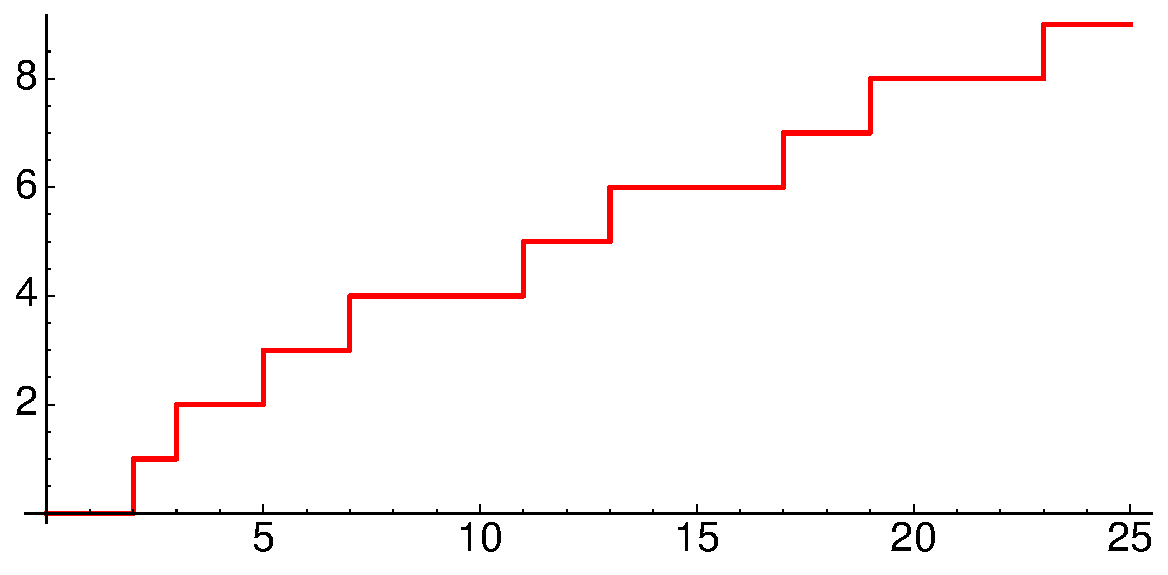
\includegraphics[width=.4\textwidth]{illustrations/PN_25} 
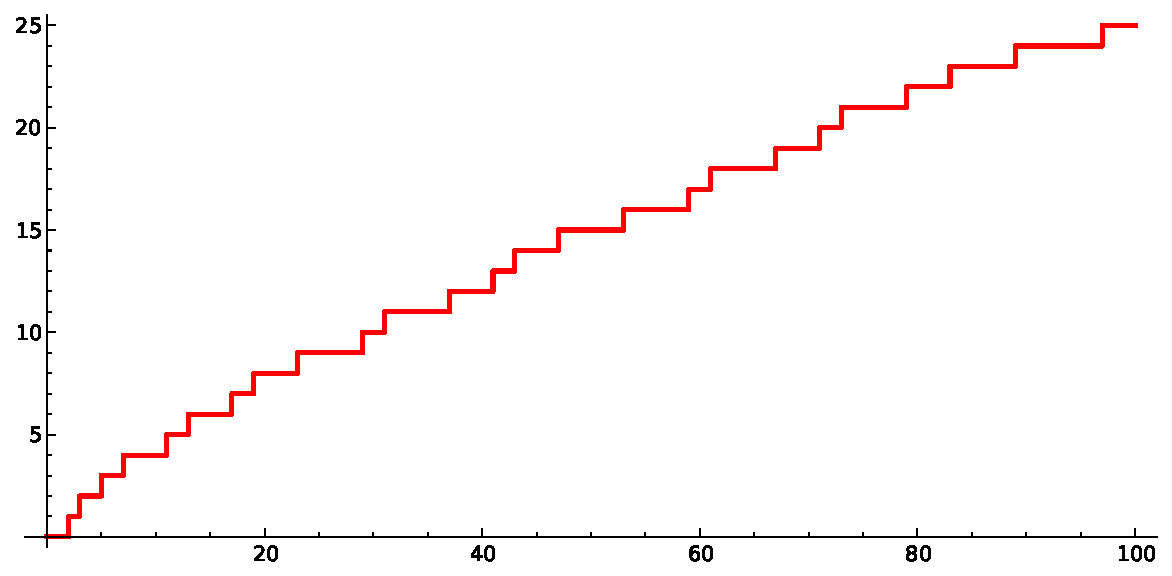
\includegraphics[width=.4\textwidth]{illustrations/PN_100}\\ 

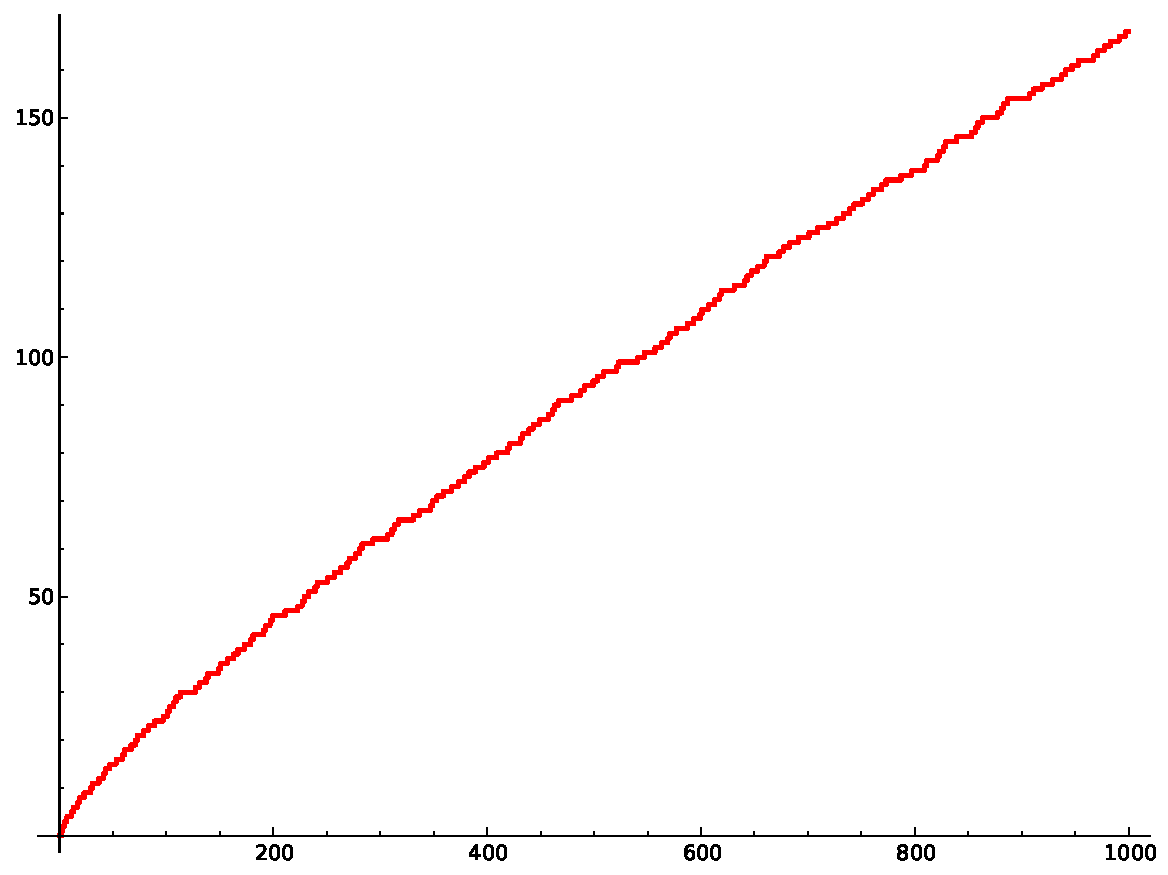
\includegraphics[width=.4\textwidth]{illustrations/PN_1000}
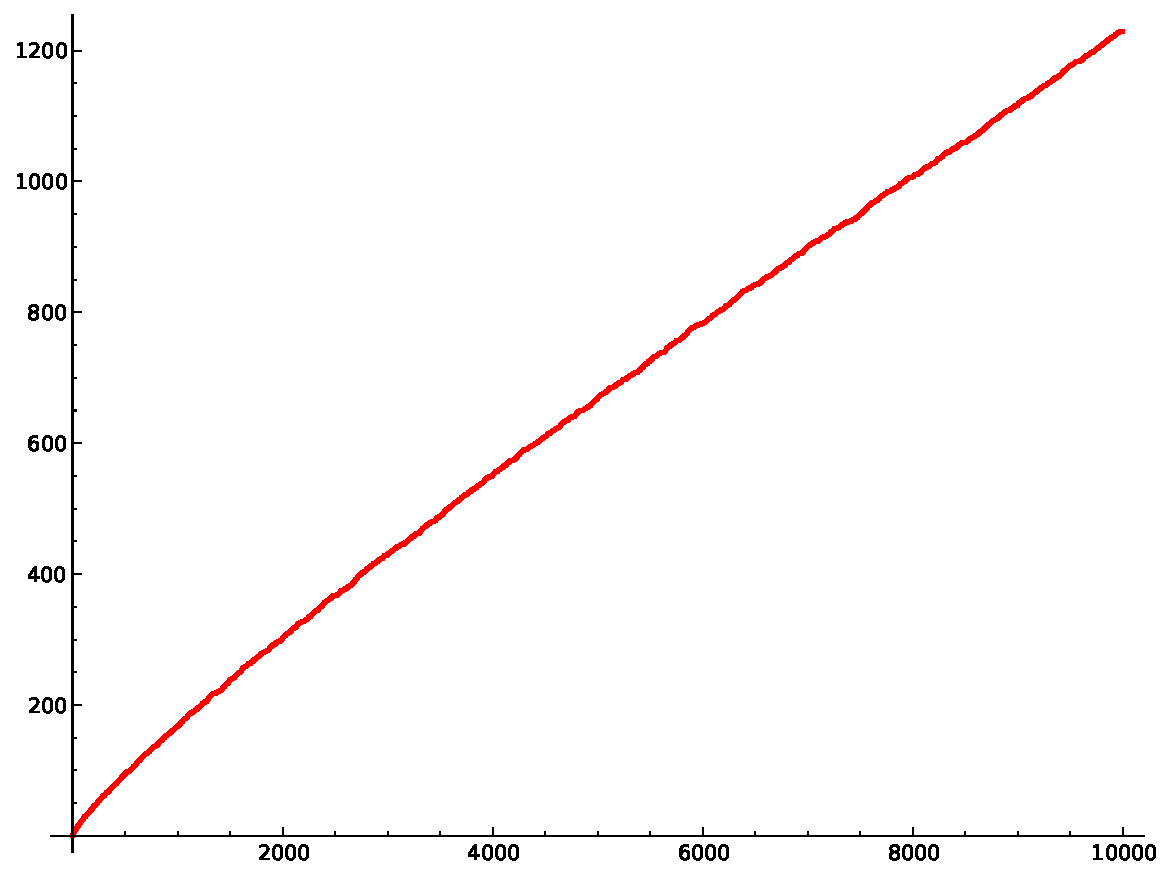
\includegraphics[width=.4\textwidth]{illustrations/PN_10000}\\ 

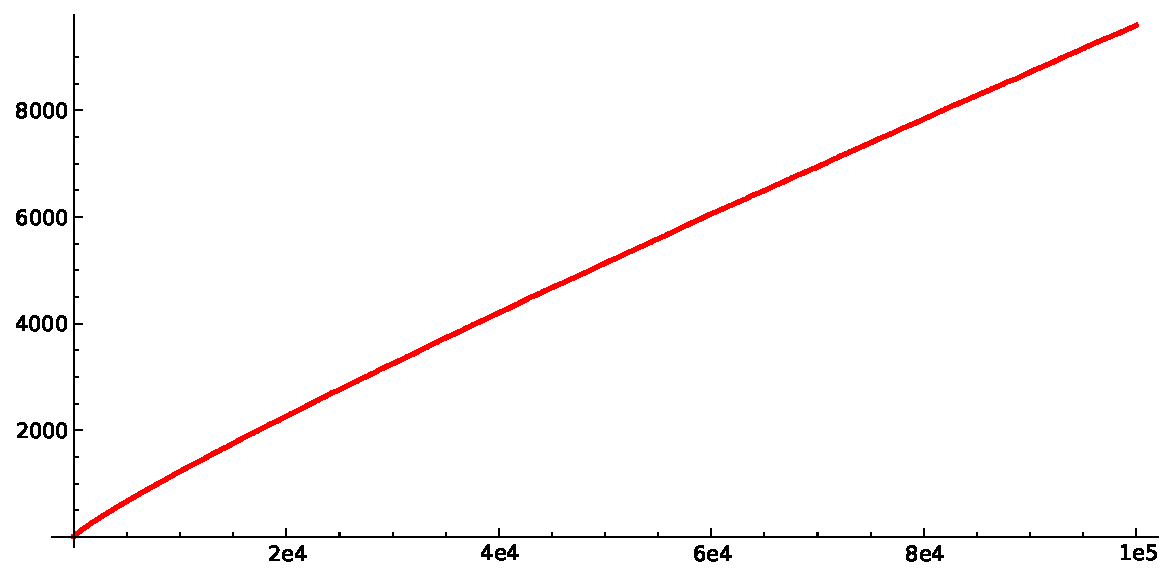
\includegraphics[width=.6\textwidth]{illustrations/PN_100000}
\end{center}
\caption{The Staircase of Primes\label{fig:staircases}}
\end{figure}

The mystery of this staircase is that the {\em information} contained
within it is---in effect---the full story of where the primes are
placed. This story seems to elude any simple description.  Can we
``tinker with'' this staircase without destroying this valuable
information?
 

\section{Tinkering with the carpentry of the staircase of primes.}

 
For starters, notice that all the {\em risers} of this staircase have
unit length. That is, they contain no numerical information except for
their placement on the $x$-axis. So, we could distort our staircase by
changing (in any way we please) the height of each riser; and as long
as we haven't brought new risers into---or old risers out
of----existence, and have not modified their position over the
$x$-axis, we have retained all the information of our original
staircase.
   
   
A more drastic-sounding thing we could do is to judiciously add new
steps to our staircase. At present, we have a step at each prime
number $p$, and no step anywhere else. Suppose we built a staircase
with a new step not only at $x=p$ for $p$ each prime number but $x =1$
and $x=p^n$ where $p^n$ runs through all powers of prime numbers as
well. Such a staircase would have, indeed, many more steps than our
original staircase had, but, nevertheless, would retain much of the
quality of the old staircase: namely it contains within it the full
story of the placement of primes {\em and their powers}.
     
A final thing we can do is to perform a distortion of the $x$-axis
(elongating or shortening it, as we wish) in any specific way, as long
as we can perform the inverse process, and ``undistort'' it if we wish.
Clearly such an operation may have mangled the staircase, but hasn't destroyed
information irretrievably.
     
We shall perform all three of these kinds of operations eventually,
and will see some great surprises as a result.  But for now, we will
perform distortions only of the first two types.  We are about to
build a new staircase that retains the precious information we need,
but is constructed according to the following architectural plan.
 
 \begin{itemize}
 
 \item We first build a staircase that has a new step precisely at $x
   =1$, and $ x= p^n$ for every {\em prime power} $p^n$ with $n\geq
   1$. That is, there will be a new step at $x= 1,2,3,4,5,8,9,11,
   \dots$
  
 \item Our staircase starts on the ground at $x=0$ and the height of the
   riser of the step at $x=1$ will be $\log(2\pi)$. The length of the
   riser of the step at $x=p^n$ will not be $1$
   (as was the length of all risers in the old staircase of primes)
   but rather: the step at $x=p^n$ will have the height of its riser
   equal to $\log p$.  So for the first few steps listed in the
   previous item, the risers will be of length $N=\log(2\pi), \log
   2,\log 3,\log 2,\log 5,\log 2,\log 3,\log 11, \dots$ These vertical
   dimensions might lead to a steeper ascent but no great loss of {\em
     information}.
  
   Although we are not quite done with our architectural work, Figure~\ref{fig:psi} shows 
   what our staircase looks like, so far.

\begin{figure}[H]
\begin{center}
\includegraphics[width=0.4\textwidth]{illustrations/psi_10}
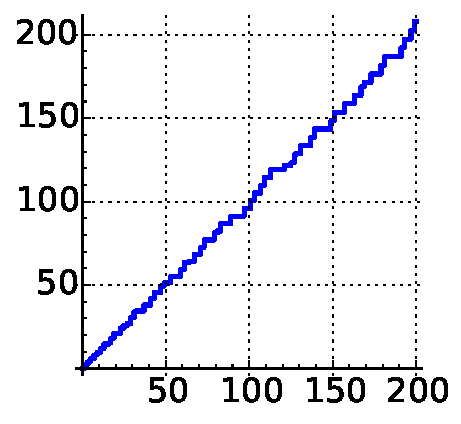
\includegraphics[width=0.4\textwidth]{illustrations/psi_200}
\caption{Illustration of the newly constructed staircase that counts weighted prime powers.\label{fig:psi}}
\end{center}
\end{figure}
  
  \end{itemize} 
  
  Notice that this new staircase looks, from afar, as if it were
  nicely approximated by the $45$ degree straight line, i.e., by the
  simple function $x$. In fact, we have---by this new
  architecture---a second {\em equivalent} way of formulating
  Riemann's hypothesis:
    
          \begin{center}
       \shadowbox{ \begin{minipage}{0.9\textwidth}
\mbox{}       \vspace{0.2ex}
       \begin{center}{\bf\large The {\bf Riemann Hypothesis} (second formulation)}\end{center}
       \medskip
       
   This new staircase is essentially square root close to the $45$
   degree straight line, i.e., to the simple function $x$.
   \vspace{1ex}
   \end{minipage}}
\end{center}

Do not worry if you do not understand why our first and second
formulations of Riemann's Hypothesis are equivalent. Our aim, in
offering the second formulation---a way of phrasing Riemann's guess
that mathematicians know to be equivalent to the first one---is to
celebrate the variety of equivalent ways we have to express Riemann's
propose answers to the question ``How many primes are there?'' and to
point out that some formulations would reveal a startling
simplicity--not immediately apparent---to the behavior of prime
numbers, no matter how erratic primes initially appear to us to
be. After all, what could be simpler than a 45 degree straight line?
 
 \bigskip


\section{What do  computer music files,  data-compression, and prime numbers have to do with each other?}

\bigskip


Sounds of all sorts---and in particular the sounds of music---travel
as vibrations of air molecules at roughly 760 miles an hour. These
vibrations---fluctuations of pressure---are often represented, or
``pictured,'' by a graph where the horizontal axis corresponds to
time, and the vertical axis corresponds to pressure at that time.  The
very purest of sounds---a single sustained note--- would look
something like this (called a ``sine wave'') when pictured (see
Figure~\ref{fig:sine}).  so that if you fixed your position somewhere
and measured air pressure due to this sound at that position, the
peaks correspond to the times when the varying air pressure is maximal
or minimal and the zeroes to the times when it is normal pressure.

\begin{figure}[H]
\begin{center}
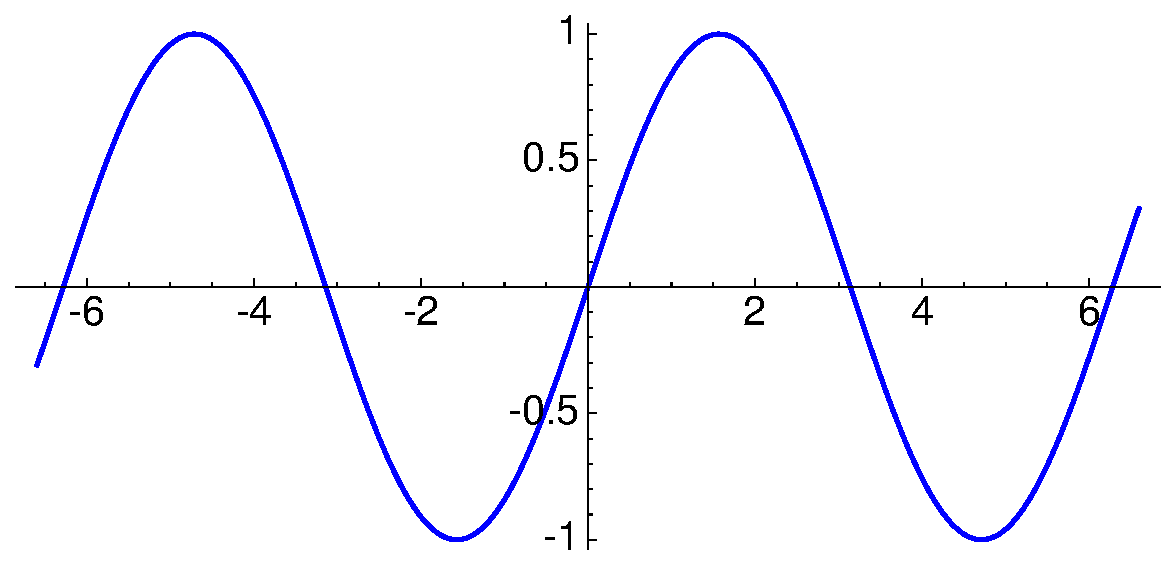
\includegraphics[width=0.6\textwidth]{illustrations/sin}  
\caption{Graph of a Sine Wave\label{fig:sine}}
\end{center}
\end{figure}  

If you want to actually hear this ``sine wave'' and other graphs,
thinking of them as ``pictures of sound,'' go to the worksheet [***].

You'll notice that there are two features to the graph in Figure~\ref{fig:sine}.

\begin{itemize}
\item {\em The height of the peaks of this sine wave:} This height is
  referred to as the {\bf amplitude} and corresponds to the {\em
    loudness} of the sound,
\item {\em The number of peaks per second:} This number is referred to
  as the {\bf frequency} and corresponds to the {\em pitch} of the
  sound.
\end{itemize}


Of course, music is rarely---perhaps never---just given by a single
pure sustained note and nothing else. A next most simple example of a
sound would be a simple chord (say a C and an E played together on
some electronic instrument that could approximate pure notes). Its
graph would be just the {\em sum} of the graphs of each of the pure
notes (see Figures~\ref{fig:sinetwofreq} and \ref{fig:sinetwofreqsum}).
    
\begin{figure}[H]
\begin{center}
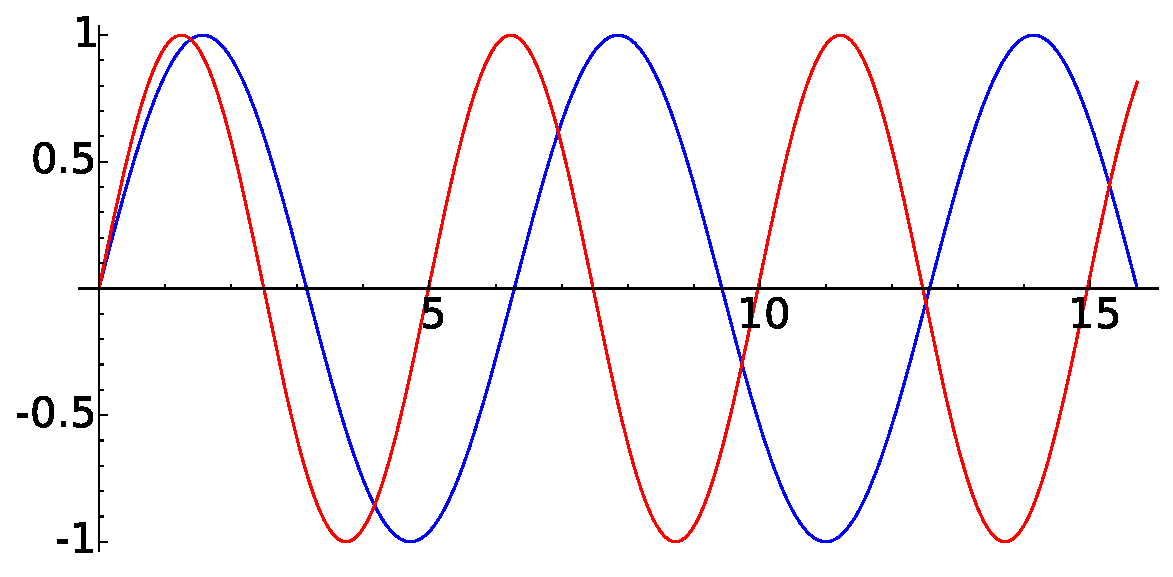
\includegraphics[width=0.6\textwidth]{illustrations/sin-twofreq}  
\caption{Graph of Two Sine Waves with Different Frequencies\label{fig:sinetwofreq}}
\end{center}
\end{figure}  

\begin{figure}[H]
\begin{center}
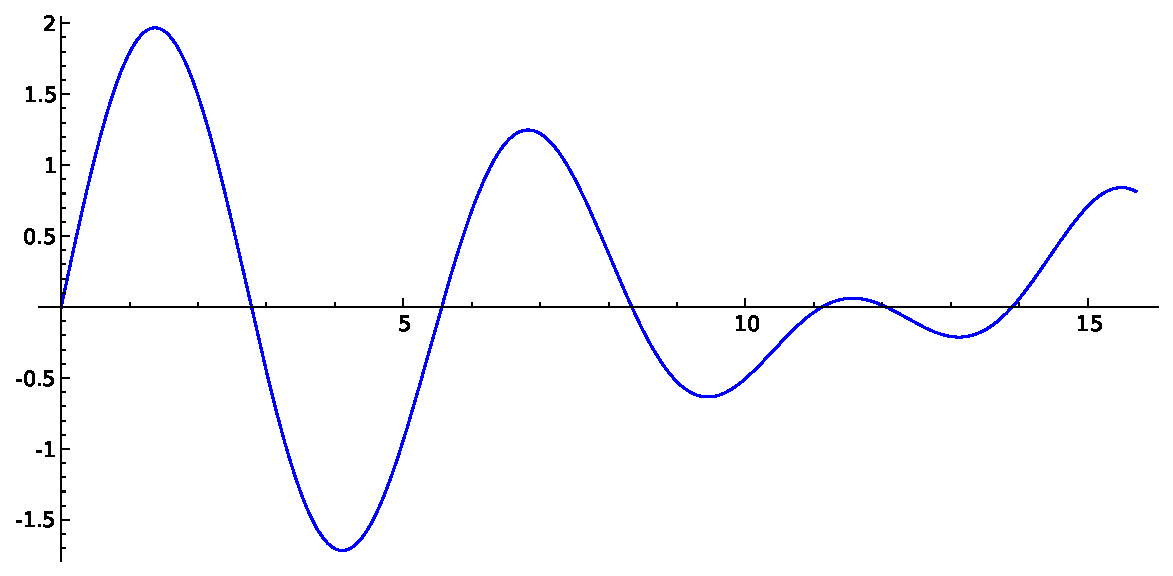
\includegraphics[width=0.6\textwidth]{illustrations/sin-twofreq-sum}  
\caption{Graph of Sum of the Two Sine Waves with Different Frequencies\label{fig:sinetwofreqsum}}
\end{center}
\end{figure}  

So the picture of the changing frequencies of this chord would be
already a pretty complicated configuration.  What we have described in
these graphs are two sine waves (our C and our E) when they are played
{\em in phase} (meaning they start at the same time) but we could
also ``delay'' the onset of the E note and play them with some
different phase relationship, for example, as illustrated
in Figures~\ref{fig:sin-twofreq-phase} and \ref{fig:sum-sin-phase}.
     
\begin{figure}[H]
\begin{center}
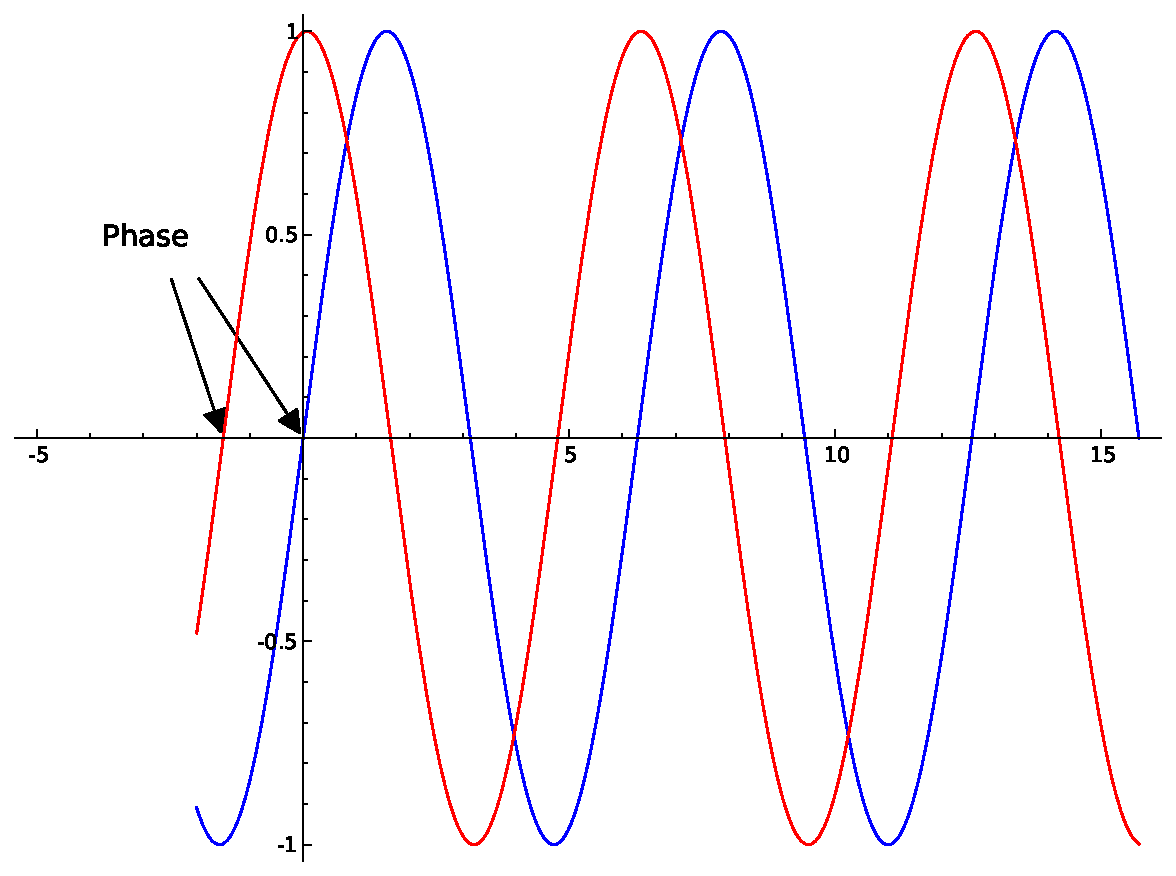
\includegraphics[width=0.6\textwidth]{illustrations/sin-twofreq-phase}  
\caption{\label{fig:sin-twofreq-phase}Graph of two ``sine'' waves in some phase relationship one to
  another [[todo: the picture should have the label {\em phase} with arrows
  showing that it is the distance between the two ``starting
  points.'']]}
\end{center}
\end{figure}  

\begin{figure}[H]
\begin{center}
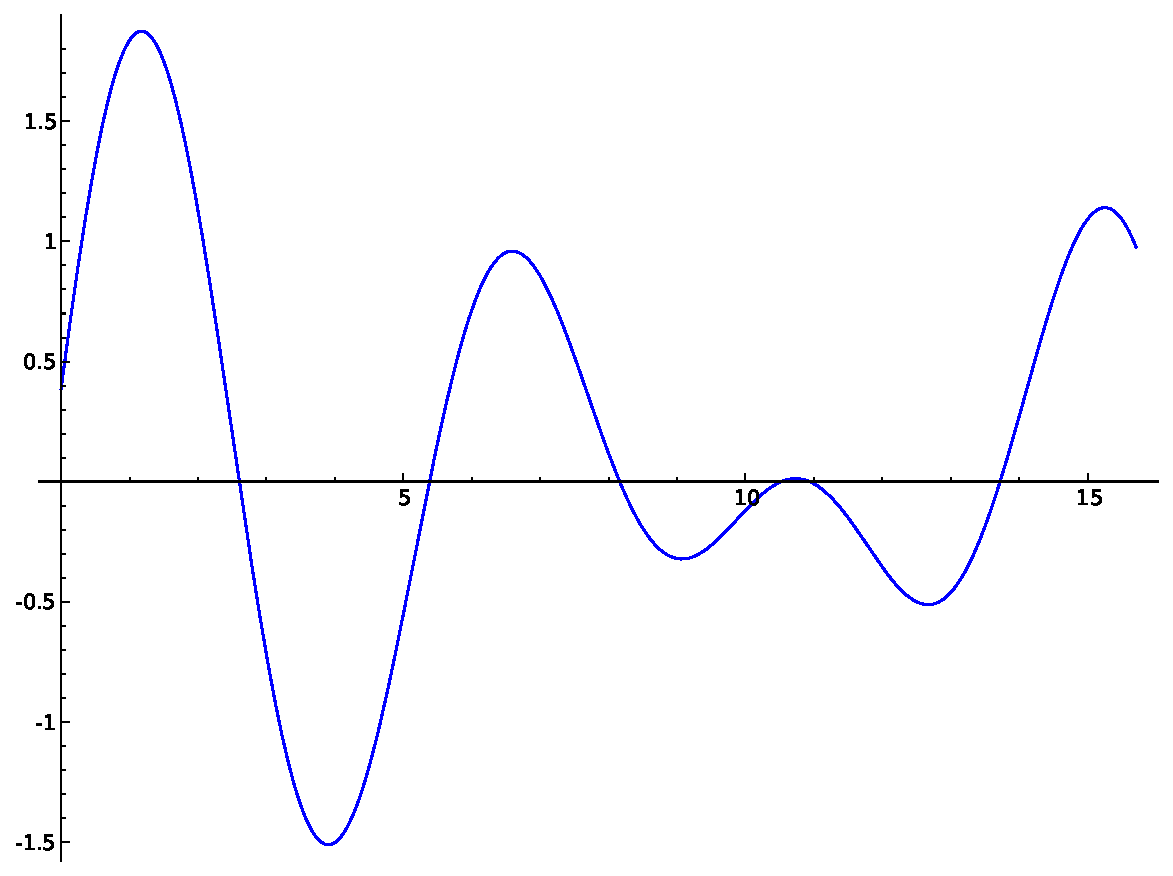
\includegraphics[width=0.6\textwidth]{illustrations/sin-twofreq-phase-sum}  
\caption{Graph of the sum of the two ``sine'' waves in some phase
  relationship\label{fig:sum-sin-phase}}
\end{center}
\end{figure}  


 
  So, {\em all you need} to reconstruct the chord graphed above is to
  know five numbers:
  \begin{itemize}
  \item the two frequencies---the collection of frequencies that make
    up the sound is called the {\em spectrum} of the sound,
  \item the {\em amplitudes} of each of these frequencies,
  \item the {\em phase} between them.
  
 \end{itemize}
 
 Now suppose you came across such a sound as pictured in
 Figure~\ref{fig:sum-sin-phase} and wanted to ``record it.''  Well,
 one way would be to sample the amplitude of the sound at many
 different times, as for example in Figure~\ref{fig:sum-sin-phase-sample}.
  
\begin{figure}[H]
\begin{center}
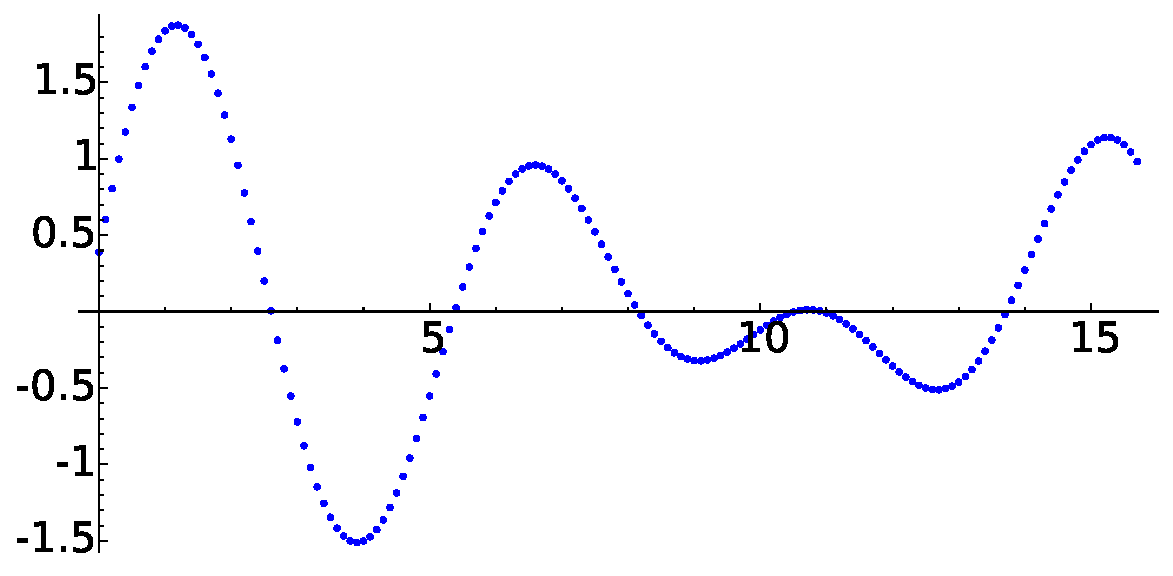
\includegraphics[width=0.6\textwidth]{illustrations/sin-twofreq-phase-sum-points}
\end{center}
\caption{Graph of sampling of a sound wave\label{fig:sum-sin-phase-sample}}
\end{figure}

Then, fill in the rest of the points to obtain Figure~\ref{fig:sum-sin-phase-sample-fill}.

\begin{figure}[H]
\begin{center}
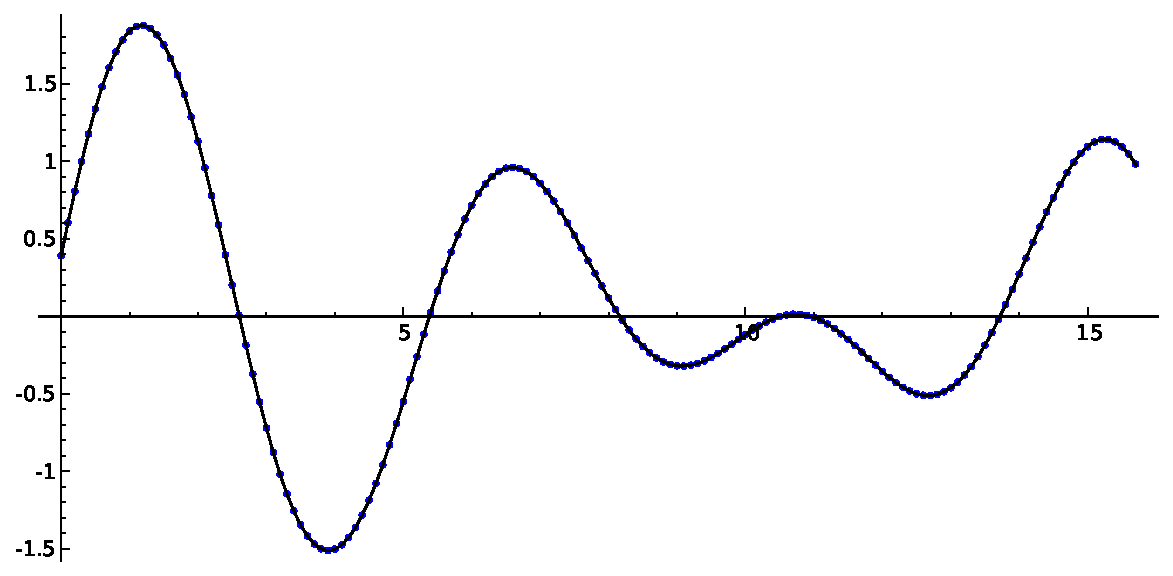
\includegraphics[width=0.6\textwidth]{illustrations/sin-twofreq-phase-sum-fill}
\end{center}
\caption{Graph obtained from Figure~\ref{fig:sum-sin-phase-sample} by
filling in the rest of the points\label{fig:sum-sin-phase-sample-fill}}
\end{figure}


But this sampling would take an enormous amount of storage space!
Current audio compact discs do their sampling 44,100 times a second to
get a reasonable quality of sound.

Another way is to simply record the {\em five} numbers: the {\em
  spectrum, amplitudes,} and {\em phase}.  Surprisingly, this seems to
be roughly the way our ear processes such a sound when we hear it.  At
this point we recommend to our readers that they download
\url{http://www.maths.abdn.ac.uk/~bensondj/html/music.pdf}, which is a
marvelous book by Dave Benson, entitled {\em Music: A Mathematical
  Offering}. This is free, and gives a beautiful account of the superb
mechanism of hearing, and of the mathematics of music.

  Even in this simplest of examples (our pure chord: the pure note C
  played simultaneously with pure note E) the {\em efficiency of data
    compression} that is the immediate bonus of analyzing the picture
  of the chords as built {\em just} with the five numbers giving {\em
    spectrum, amplitudes,} and {\em phase} is staggering.

\ill{fourier}{0.3}{Jean Baptiste Joseph Fourier (1768--1830)}

This type of analysis, in general, is called {\em Fourier Analysis}
and is one of the glorious chapters of mathematics.  One way of
picturing {\em spectrum} and {\em amplitudes} of a sound is by a bar
graph which might be called the {\em spectral picture} of the sound,
the horizontal axis depicting frequency and the vertical one depicting
amplitude: the height of a bar at any frequency is proportional to the
amplitude of that frequency ``in'' the sound.
 
So our CE chord would have the spectral picture in
Figure~\ref{fig:ce-spectral}.
 
\begin{figure}[H]
\begin{center}
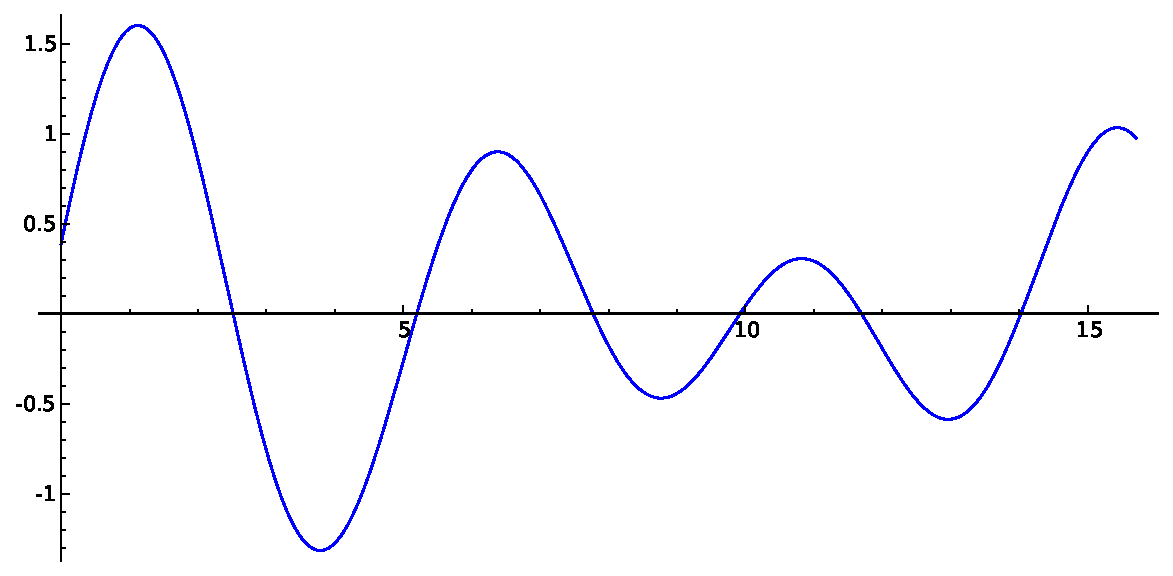
\includegraphics[width=0.4\textwidth]{illustrations/sound-ce-general_sum}
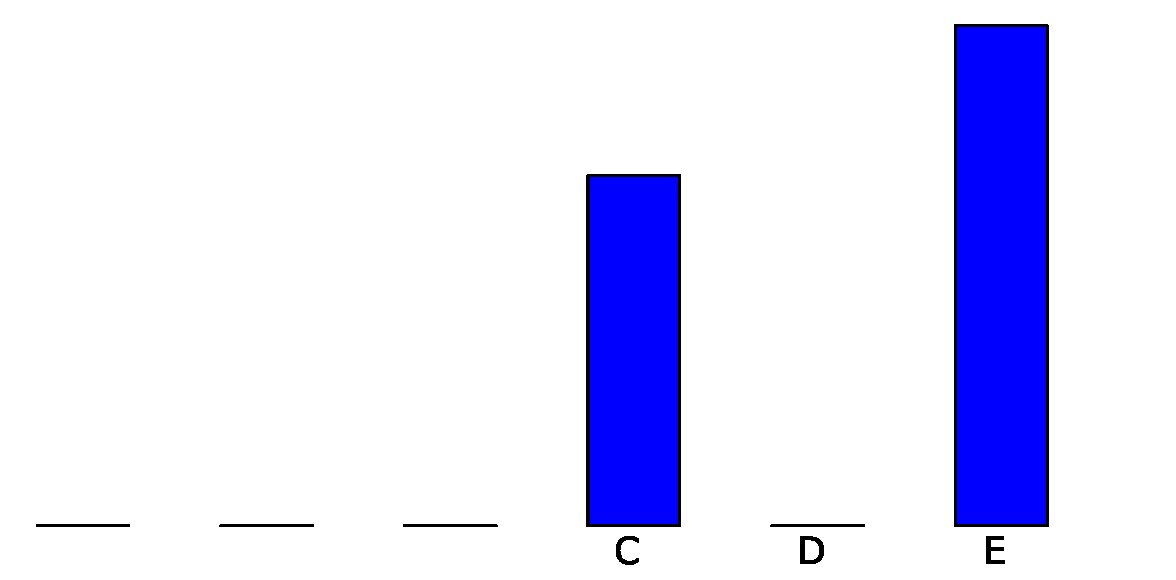
\includegraphics[width=0.4\textwidth]{illustrations/sound-ce-general_sum-blips}
\end{center}
\caption{Spectral Picture of a CE chord\label{fig:ce-spectral}}
\end{figure}

This spectral picture ignores the phase but is nevertheless a very
good portrait of the sound.  The spectral picture of a graph gets us
to think of that graph as ``built up by the superposition of a bunch
of pure waves,'' and if the graph is complicated enough we may very well
need {\em infinitely} many pure waves to build it up!  Fourier analysis is a
mathematical theory that allows us to start with any graph---we are
thinking here of graphs that picture sounds, but any graph will do---
and actually compute its spectral picture (and even keep track of
phases).
 
 
The operation that starts with a graph and goes to its spectral
picture that records the frequencies, amplitudes, and phases of the
pure sine waves that, together, compose the graph is called the {\em
  Fourier transform} and nowadays there are very fast procedures for
getting accurate {\em Fourier transforms} (meaning accurate spectral
pictures including information about phases) by computer.\endnote{Discuss
some good readable article on the Fast Fourier Transform algorithm; there are probably many such algorithms.}
 
 
If you pass to the worksheet at this point, you'll be able to see the
Fourier transforms of many different sounds, and experiment for
yourself.  The theory behind this operation (Fourier transform giving
us a spectral analysis of a graph) is quite beautiful, but equally
impressive is how---given the power of modern computation---you can
immediately perform this operation for yourself to get a sense of how
different wave-sounds can be constructed from the superposition of
pure tones.  You can do this now!  (Go to [**].)  For example if you
want to hear what a {\em sawtooth} wave sounds like, as in
Figure~\ref{fig:sawtooth}, 
   
   
\begin{figure}[H]
\begin{center}
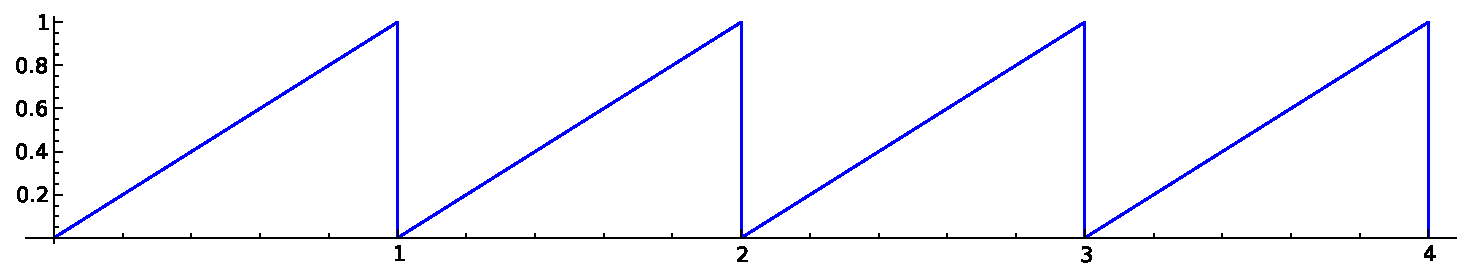
\includegraphics[width=0.7\textwidth]{illustrations/sawtooth}
\end{center}
\caption{Graph of Sawtooth Wave\label{fig:sawtooth}}
\end{figure}

\noindent just go to the worksheet; if you want to know its spectral picture, click on the Fourier transform operator to get Figure~\ref{fig:sawtooth-spectrum}:
    
 \bigskip


\begin{figure}[H]
\begin{center}
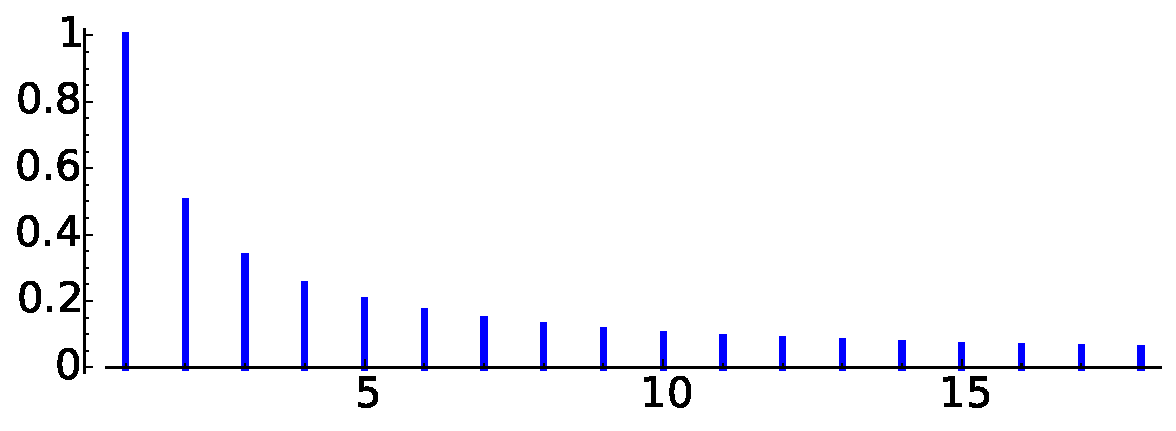
\includegraphics[width=0.6\textwidth]{illustrations/sawtooth-spectrum}
\end{center}
\caption{The Spectrum of the Sawtooth Wave Has a Spike of Height $1/k$ at 
each integer $k$\label{fig:sawtooth-spectrum}}
\end{figure}
  

       
\begin{figure}[H]
\begin{center}
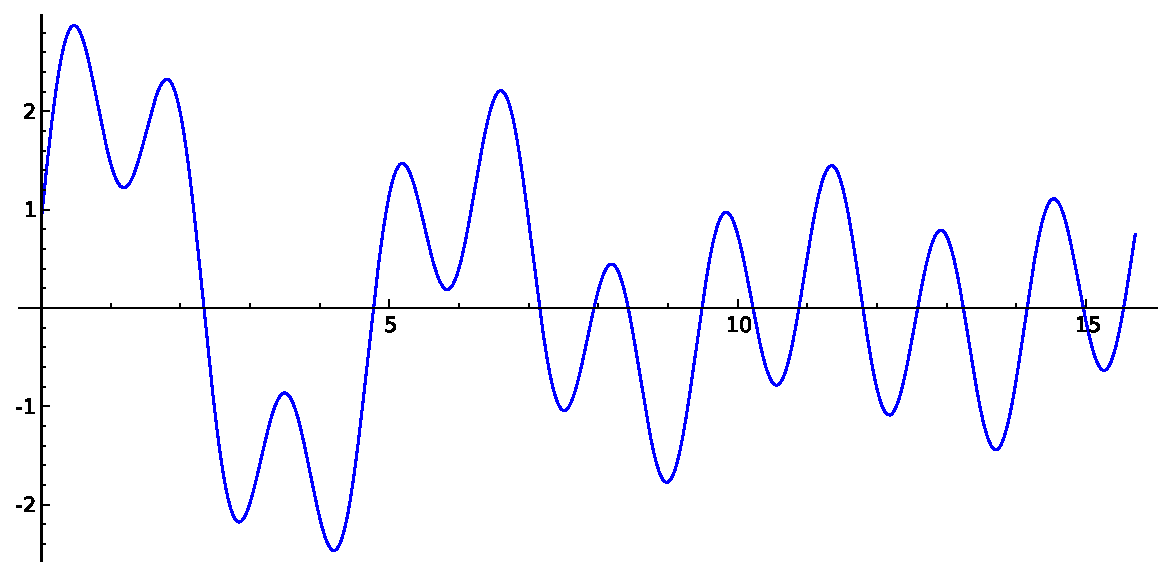
\includegraphics[width=0.6\textwidth]{illustrations/complicated-wave}
\end{center}
\caption{A Complicated Sound Wave\label{fig:complicated-wave}}
\end{figure}
Suppose you have a complicated sound wave, say as in
Figure~\ref{fig:complicated-wave}, and you want to record it.
Standard audio CD's record their data by intensive sampling as we
mentioned. In contrast, current mp3 audio compression technology uses
Fourier transforms plus sophisticated algorithms based on
psycho-acoustic understanding. With this, mp3 technology manages to
get a compression factor of 8--12 with little {\em perceived} loss in
quality.
 
\begin{figure}[H]
\begin{center}
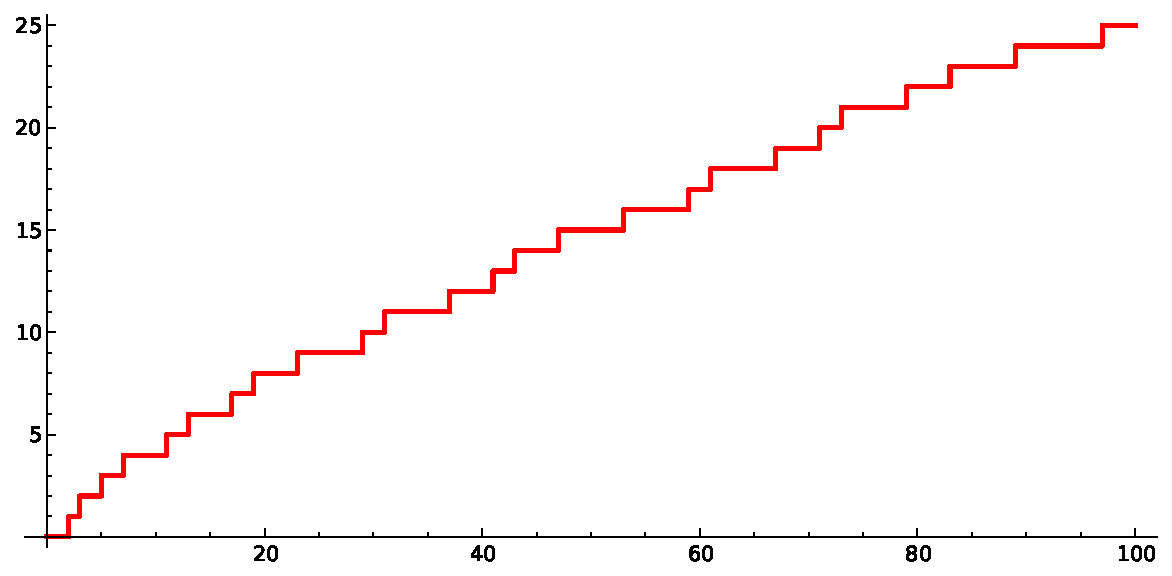
\includegraphics[width=.35\textwidth]{illustrations/PN_100}
\caption{The Staircase of Primes\label{fig:staircase100}}
\end{center}
\end{figure}

Is there a way of using Fourier Analysis to re-express the complicated
picture of the staircase of primes (or, perhaps, something
  that contains the same basic information as that staircase).
(Figure~\ref{fig:staircase100}) in a data-compressed way as a sum of
pure ``sine waves?''  Does this ornery staircase of primes have a
spectrum that we can compute, just as we have done for the saw-tooth
wave above, or for the major third CE chord?  And will that spectrum
show us {\em order} and {\em profound organization} lurking within the
staircase?  Will our understanding of the spectrum allow us to
reproduce all the pertinent information about the placement of primes
among all whole numbers, elegantly and {\em faithfully}?  Of course,
here we would not settle for ``little loss of quality." We would want,
in the end, a perfect recording!
  
 
These queries represent some of the aspirations that we are tempted to
have, as we follow through on Riemann's view. Strangely enough, it is
towards questions like these that Riemann's Hypothesis may take us. We
began with the simple question about primes: {\em how to count them},
and are led to ask for profound, and hidden, regularities in
structure.

\section{ To our readers of Part I. } 
The statement of the Riemann Hypothesis---admittedly as elusive as
before---has, at least, been expressed elegantly and more simply,
given our new staircase that approximates (conjecturally with {\em
  essential square root accuracy}) a 45 degree straight line.
   
We have offered two equivalent formulations of the Riemann Hypothesis,
both having to do with the manner in which the prime numbers are
situated among all whole numbers.

In doing this, we hope that we have convinced you that---in the words
of Don Zagier---primes seem to obey no other law than that of chance
and yet exhibit stunning regularity.  This is the end of part I of our
booklet, and is largely the end of our main mission, to explain---in
elementary terms---{\em what is Riemann's Hypothesis?}
    
     
For readers who have studied Differential Calculus and who are happy
with complex numbers, we shall go further and show that the pursuit of
Riemann's hypothesis may provide a key to some deeper structure of the
prime number, and to the nature of the laws that they obey.


       
\bigskip   
\bigskip   
\bigskip   
\bigskip   
\centerline{\Large\bf Part II }
    
\bigskip 
\section{How Calculus manages to find the slopes of graphs that  
have no slopes}   
   
Differential Calculus, initially the creation of Newton and/or
Leibniz, acquaints us with {\em slopes} of graphs,
   

[[Is the following a suggestion to replace the picture below by something with a log function?  I don't remember what the point of this querry is: {\em a graph that is more of a log with a question: ``What is the slope
of the tangent line?'' answer: ``here it is''; How compute?  this is
calculus.}]] 
   
   
\ill{graph_slope_deriv}{0.5}{A picture of a graph of a function (blue), a slope at a point (green), and the graph of the derivative (red).}
      
\noindent Calculus explains to us how to calculate those slopes, and
finally, shows us the power that we then have to answer problems we
could not answer if we couldn't compute those slopes.


Usually, in elementary Calculus classes we are called upon to compute
slopes only of smooth graphs, i.e., graphs that actually {\em have}
slopes at each of their points, such as in the illustration just
above.  What could Calculus possibly do if confronted with a graph
that has {\em jumps}, such as in Figure~\ref{fig:jump}.
 
\ill{jump}{0.5}{A graph that jumps---it is $1$ up to $3$ and then $2$ after that point\label{fig:jump}}
  
The most comfortable way to deal with the graph of such a function is
to just approximate it by a nice smooth function as in
Figure~\ref{fig:jumpsmooth}.
    
   
\ill{jump-smooth}{0.5}{A picture of a smooth graph approximating the
  graph that is $1$ up to some point $x$ and then $2$ after that
  point, the smooth graph being flat mostly.\label{fig:jumpsmooth}}


Then take the {\em derivative} of that smooth function.  Of course,
this is just an approximation, so we might try to make a better
approximation, which we do in each successive graph starting
with Figure~\ref{fig:derivsmoothapprox} below.


\ill{jump-smooth-deriv-point700000000000000}{0.6}{A picture of the derivative of
a smooth approximation to a function that jumps.}

Note that---as you would expect---in the range where the initial
function is constant, its derivative is zero. In the subsequent
figures, our initial function will be {\it nonconstant} for smaller
and smaller intervals about the origin. Note also that, in our series
of pictures below, we will be successively rescaling the $y$-axis; all
our initial functions have the value $1$ for ``large" negative numbers
and the value $2$ for large positive numbers.

\ill{jump-smooth-deriv-point200000000000000}{0.5}{Second picture of the derivative of
a smooth approximation to a function that jumps.}
\ill{jump-smooth-deriv-point0500000000000000}{0.5}{Third picture of the derivative of
a smooth approximation to a function that jumps.}
\ill{jump-smooth-deriv-point0100000000000000}{0.5}{Fourth picture of the derivative of
a smooth approximation to a function that jumps.}


Notice, what is happening: as the approximation gets better and
better, the derivative will be zero mostly, with a blip at the point
of discontinuity, and the blip will get higher and higher.  Now, early
mathematicians (Newton, Leibniz)---in replacing approximate speeds by
instantaneous velocities by {\em passing to limits}---had to wait a
while before later mathematicians (e.g., Weierstrass) gave a rigorous
foundation for what they were doing.  Happily however, this process we
are discussing, of approximating discontinuous functions more and more
exactly by smooth functions, and taking their derivatives to get the
blip-functions as we have just seen in the graphs above led
mathematicians (notably the French mathematician, Laurent Schwartz) to
provide a mathematically rigorous foundation (that we needn't go into
here) called the {\em theory of distributions.} Thanks to this theory
you can, so to speak, {\em go all the way} to form what you can
legitimately call the {\em derivative} of the function that is $0$
before the point $x$ and $1$ afterwards; if we were to think of this
as a {\em function} we would be in trouble: it would have $\infty$ as
a value at $x$, and---worse---it would be no use to us. But the modern
remedy is to formulate a conceptual context in which it has a genuine
existence, and can be genuinely used in exactly the same way as the
derivatives of smooth functions are used. The only change here is that
the derivative of this discontinuous function has a status, not as a
function, but rather as a {\em distribution}.  

\section{Distributions: sharpening our approximating functions even if
  we have to let them shoot out to infinity}
These ``blip-functions'' as we have been referring to them are more
officially called {\em Dirac $\delta$-functions}, the adjective
``Dirac'' being in honor of the physicist who first worked effectively
with this concept, the $\delta$ being the symbol he assigned to these
objects, and the noun ``function'' should properly be in
quotation-marks for---properly speaking the Dirac $\delta$-function is
not---as we have explained above---a bona fide function but rather a
{\em distribution}.

\ill{dirac}{0.2}{Paul Adrien Maurice Dirac (1902--1984)}

   The curious aspect of the Dirac $\delta$-function that has its blip
   at the point $x$ is that it is flatly {\em zero} in any interval in
   the $t$-line that doesn't include the point $t=x$.  We say that
   this Dirac $\delta$-function has its {\bf support} at the point $x$.

\endnote{
[[I found this comment about ``Generalized functions"
     (which seems to be an early name for distributions) on Wikipedia:

\vskip10pt
\begin{quote} ``Generalized functions" were introduced by Sergei Sobolev in 1935. They were independently introduced in the late 1940s by Laurent Schwartz, who developed a comprehensive theory of distributions."
\end{quote}

so maybe we should look into the history of this. (But I'm not keen on
getting too much into it: just if we need to add a short end-note
about it, to credit Sobolev $\dots$)]]
}

\section{Finding the slopes of staircases} 

[[I also think that there should be an ``introductory" simpler picture
as well (simpler than, say, figure 18.2) where we have the staircase
of primes between $1$ and $10$ and give the derivative for
that---which just has four blips, and then move to the fuller figure
18.2]]

\begin{figure}[H]
\begin{center}
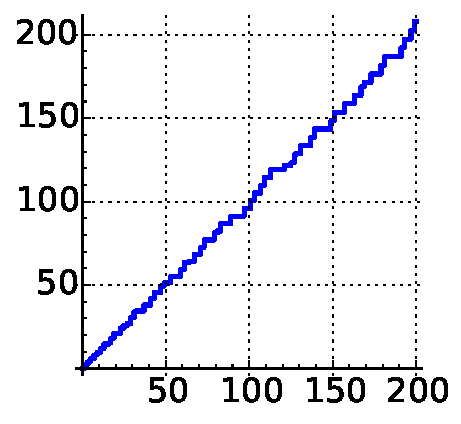
\includegraphics[width=0.7\textwidth]{illustrations/psi_200}
\caption{Illustration of the  staircase $\Psi(x)$  constructed in Part I that 
counts weighted prime powers.\label{fig:psi_200}}
\end{center}
\end{figure}
  
So what happens when we take the derivative---in the sense of
distributions---of a complicated staircase?  For example, see
Figure~\ref{fig:psi_200}.  Well, we would have blip-functions (alias:
Dirac $\delta$-functions) at each point of discontinuity of $\Psi(x)$;
that is, at $x=$ any power of a prime.
  
     \bigskip
   
     \ill{psi_prime}{.7}{Continuous approximation to the staircase
       $\Psi(x)$ (in red) along with a plot (in blue) of the
       derivative of this approximation.}
      
\bigskip

[[Barry: I think that I'd like to add a philosophical paragraph
(short, I promise) about performing mathematical changes that ``lose
no information."  OK. So I don't forget this, I'll call it LNI for
``lose no information" and will try to write it.]]
  
As we have hinted above, we lose no information if we further modify
our staircase by distorting the $x$-axis, replacing $x$ by $e^t$ (as
long as we {\em remember what it is we have done!})  so---for reasons
that we will {\em only} see after the next section---we reconfigure
our distribution $\Psi'(x)$ replacing it with the distribution

$$
  \Phi(t) : = \Psi'(e^t)/e^{\frac{t}{2}}.
$$

  
\bigskip
   
   
\ill{phi_50}{0.6}{An approximation to the distribution $\Phi(t)$}
     
\bigskip


This distribution $\Phi(t)$ has a ``blip'' at $t=0$ and also at each
positive multiple of $\log p$ as $p$ runs through the primes.  It has
its {\em support} at the discrete set of points $t=0$ and $t=$
integer multiples of $\log p$ as $p$ runs through the primes.


We will refer to distributions with discrete support as {\bf spike
  distributions} because graphs of functions that approximate them
look like they have {\em spikes} around the points in their support.

The spike distribution $\Phi(t)$ is now a major player in our drama,
because all of the crucial valuable information of placement of primes
is contained in it: the ``blips'' constituting this distribution (its
support) would allow us to reconstruct the position of the prime
numbers among all numbers.

But there are many other ways to package this vital information, so we
must explain our motivation for subjecting our poor initial staircase
to the particular series of brutal acts of distortion that we
described, that end up with the distribution $\Phi(t)$.

We do this because we are fascinated by this list of very surprising
facts about this $\Phi(t)$, a distribution that contains full
information about the placement of prime numbers among all numbers.

\begin{itemize}
\item The first surprising thing about this discrete distribution is that its Fourier transform is again discrete. 
\vskip20pt

[[Put an array of say 6 random plots of discrete distributions along
with their fft's which don't look discrete at all.]]  In
Section~\ref{sec:dd} we will revisit the curious case of distributions
with discrete support that have Fourier transforms with discrete
support.

\vskip20pt
That is, the spectrum is given by an infinite, but discrete list of
numbers at the spikes down in Figure~\ref{fig:phi_even_a}.
$$
  \theta_1, \theta_2, \theta_3,\dots
$$

This, Riemann knew!  

An endnote -- decide where to hang this.\endnote{  
{\bf Spike distributions that have discrete spectrum}
    
{\bf Aside.  Here we talk about distributions with discrete support; a
  'spike distribution' is then a sum of $\delta$-distributions
  supported on a discrete set of points.  We talk about the curious
  situation where the Fourier transform of one of these is again one,
  with a few clean examples.  We note that any spike distribution that
  has the property that its Fourier transform is again a spike also
  has the curious ``error-correcting virtue'' that if you ever forget
  a finite number of points of its support you can retrieve them.  We
  need really interesting SAGE worksheets here.}
      
      
{\bf The Spike distribution $\Phi(t)$; the Riemann Hypothesis
  ({\em third formulation})}
  
Here we use the basic definition of Fourier transform, and get by
simple integration that the even Fourier transform of $\Phi(t)=
\Psi'(e^t)/e^{t/2}$ is given by the distribution defined by the
formula
$${\hat \Phi}_{\rm even}(s): = \sum_{p^n} {\frac{\log(p)}{p^{n/2}}}\cos(ns \log(p))$$ 
and the odd Fourier transform is
$${\hat \Phi}_{\rm odd}(s): = \sum_{p^n} {\frac{\log(p)}{p^{n/2}}}\sin(ns \log(p)).$$
   
   
Figures~\ref{fig:phi_even} and \ref{fig:phi_odd} show what you get for
graphs of these distributions ${\hat \Phi}_{\rm even}(s)$ and ${\hat
  \Phi}_{\rm odd}(s)$ if you cut off the sums above at $p^n < 100$.
  
\begin{figure}[H]
\begin{center}
\includegraphics[width=0.7\textwidth]{illustrations/phi_even}
\caption{Graph of an approximation to ${\hat \Phi}_{\rm even}(s)$ using $p^n<100$\label{fig:phi_even}}
\end{center}
\end{figure}
  
\begin{figure}[H]
\begin{center}
\includegraphics[width=0.7\textwidth]{illustrations/phi_odd}
\caption{Graph of an approximation to ${\hat \Phi}_{\rm odd}(s)$ using $p^n<100$\label{fig:phi_odd}}
\end{center}
\end{figure}
   

{\bf [Barry: I've been trying the below and numerically it seems that
  it just doesn't work.  The issue is likely roundoff error, so I
  suggest not doing this.]  William: We could show a series of better
  and better approximations to the even and odd Fourier transforms of
  $\Phi(t)$, noting that the approximations to even one seem to be
  coalescing to spikes at (or around, at least) the real numbers
  $14.13...$ etc.  and the approximations to the odd one seems to have
  some strange behavior at those same real numbers $14.13...$ etc.
  but could very well be settling down to zero. We then blurt out that
  this is---in fact---the case, and is proven (we should check that
  we're not overstating things, but then:}
  
Define the {\bf Spectrum of the Primes} the set of real numbers
$\theta_1, \theta_2, \theta_3, \dots$ that comprise the {\em support}
of the blip distribution ${\hat \Phi}_{\rm even}(s)$.
 
 
 \begin{center}
      \shadowbox{ \begin{minipage}{0.9\textwidth}
      \mbox{}       \vspace{0.2ex}
      \begin{center}{\bf\large The Riemann Hypothesis is equivalent to the assertion that  $\Phi(t)$ is {\em equal to} the distribution defined as the summation $1+\sum_{i=1}^{\infty}\cos(\theta_i t)$}  where the $\theta_i$'s run through the spectrum of the primes. \end{center}
...
    \vspace{1ex}
    \end{minipage}}
 \end{center}
\bigskip

 
{\bf Aside. Here we will motivate the above equivalent statement of RH
  (that $\phi(t)$ is a sum of the $\cos(\theta t)$'s for a discrete
  set $\Theta$ of $\theta$'s. Discuss this amazing feature. Discuss
  that if $\Theta$ exists at all, i.e., if RH is true, $\Theta$ has
  the ``error-correcting virtue.'' We begin to compute it in a
  ``worksheet'' given knowledge of the primes, and we wonder whether we
  can find any other (nonbanal, of course) discrete set $\Theta'$ that
  has the property that the sum of the $\cos(\theta' t)$'s for
  $\theta' \in \Theta'$ is discrete.}

\bigskip

\ill{cos_sum_1_30}{.8}{Illustration of $-\sum_{i=1}^{1000} \cos(s\theta_i)$, where
$\theta_1 \sim 14.13, \ldots$ are the first $1000$ frequencies.  The red
dots are at the prime powers $p^n$, whose size is proportional to $\log(p)$.}

\ill{sum_cos_28_34}{.8}{Illustration of $-\sum_{i=1}^{1000} \cos(s\theta_i)$ in the
neighborhood of a twin prime.  Notice how the two primes $29$ and $31$ are separated out
by the Fourier series, and how the prime power $2^5$ appears.}

\ill{sum_cos_spike_plot_1000}{.7}{Fourier series illustration from $1000$ to $1030$}

\ill{sum_cos_fourier_transform_near_100}{.8}{The Fourier transform of the distribution 
    supported on prime powers, i.e., which is $\delta \frac{\log(p)}{p^{n/2}}$ at the
    prime power $p^n$.}
    
   \bigskip 
  
%\section{Approximations versus exact descriptions: the spectral analysis of primes }

%{\bf Aside. We give a ``Fourier'' reconstruction of $\psi(t)$ in terms of $\Theta$}
 
 \ill{psi_just_waves1}{0.7}{Illustration of 
$\displaystyle\frac{\theta\sin(t\theta) + \frac{1}{2}\cos(t\theta)}{\theta^2 + 1/4}$,
for $\theta\sim 14.13$,  which is the 
wave component of the first Fourier approximation to $\Phi(t)$}

\ill{psi_2_waves}{.7}{The first two wave components that appear in the Fourier series of $\Phi(t)$,
are $\frac{\theta\sin(t\theta) + \frac{1}{2}\cos(t\theta)}{\theta^2 + 1/4}$
for $\theta \sim 14.13, 21.02$}

\ill{psi_with_first_zero}{.5}{The first term of the Fourier series of $\Phi(t)$ is $\displaystyle  
          \frac{e^{t/2} \theta \sin(t\theta) + \
                    \frac{1}{2} e^{t/2} \cos(t\theta)}{\theta^2 + 1/4} $, 
          where $\theta \sim 14.134725$}
          
\ill{psi_with_exp_2}{.7}{The first two components of the Fourier series 
of $\Phi(t)$ (including the exponential factors) are
$e^{t/2} \cdot \frac{\theta\sin(t\theta) + \frac{1}{2}\cos(t\theta)}{\theta^2 + 1/4}$
for $\theta \sim 14.13, 21.02$}

\ill{psi_approx_1_2_5_30}{0.7}{Fourier approximations to the step function 
$\Psi$ obtained using $1$, $2$, $5$, and $30$ frequencies.}

\ill{psi_approx_using_30_zeros_from4to5}{0.7}{Fourier 
approximation to the step function $\Psi$ obtained using $30$
frequences and graphed from $1$ to $5$}

\ill{psi_using_30_terms}{0.7}{Fourier approximation to the step 
function $\Psi$ obtained using $30$ frequences.}
}
%%%%%%%%%%%%%%%%%%%%%%%%%%%%%%%%%%%%%%%

\begin{figure}[H]
\begin{center}
\includegraphics[width=0.5\textwidth]{illustrations/phi_even}
\caption{Approximation of (even) Fourier transform of $\Phi(t)$ using prime powers $<100$\label{fig:phi_even_a}}
\end{center}
\end{figure}


\item

 We can---at least approximately---{\it compute} the $\theta_i$'s of this spectrum. Riemann knew how to compute too!  In fact, he computed to pretty good accuracy, the first few $\theta_i$'s:
\begin{eqnarray*}
\theta_1 &=& 14.134725 \dots\\
\theta_2 &=& 21.022039 \dots\\
\theta_3 &=& 25.010857 \dots\\
\theta_4 &=& 30.424876 \dots\\
\theta_5 &=& 32.935061 \dots\\
\theta_6 &=& 37.586178 \dots
\end{eqnarray*}

[[Put an image from Riemann's manuscript.  Actually, I just looked
and there are no explicit zeros in Riemann's 1859 manuscript.  Is
there some other scan you have that has him finding zeros?
Barry -- where is this?  I looked carefully
through Riemann's paper where he introduces Zeta, and there are no
explicit zeros there.  Maybe somewhere else?
]]

\begin{quote}
  ``One now finds indeed approximately this number of real roots
  within these limits, and it is very probable that all roots are
  real. Certainly one would wish for a stricter proof here; I have
  meanwhile temporarily put aside the search for this after some
  futile attempts, as it appears unnecessary for the next objective of
  my investigation.''

-- Riemann, 1859
\end{quote}

Nowadays, these mysterious numbers, these spectral lines for the
staircase of primes are known to great accuracy.  Here is the smallest
one, $\theta_1$, given with over $1,\!000$ digits of its decimal
expansion: \vskip20pt 

$14.134725141734693790457251983562470270784257115699243175685567460149\newline
9634298092567649490103931715610127792029715487974367661426914698822545\newline
8250536323944713778041338123720597054962195586586020055556672583601077\newline
3700205410982661507542780517442591306254481978651072304938725629738321\newline
5774203952157256748093321400349904680343462673144209203773854871413783\newline
1735639699536542811307968053149168852906782082298049264338666734623320\newline
0787587617920056048680543568014444246510655975686659032286865105448594\newline
4432062407272703209427452221304874872092412385141835146054279015244783\newline
3835425453344004487936806761697300819000731393854983736215013045167269\newline
6838920039176285123212854220523969133425832275335164060169763527563758\newline
9695376749203361272092599917304270756830879511844534891800863008264831\newline
2516911271068291052375961797743181517071354531677549515382893784903647\newline
4709727019948485532209253574357909226125247736595518016975233461213977\newline
3160053541259267474557258778014726098308089786007125320875093959979666\newline
60675378381214891908864977277554420656532052405$

\vskip20pt
\noindent and if, by any chance, you wish to peruse the first
$100,\!000$ of these $\theta_i$'s lovingly calculated to an accuracy
within $3\cdot 10^{-9}$, consult Andrew Odlyzko's tables:
\url{http://www.dtc.umn.edu/~odlyzko/zeta_tables}

\item Better yet, we can compute this spectrum in terms of the {\it
    zeroes} of the famous function of a complex variable, known as
  {\it Riemann's zeta-function}, the function we mentioned in passing
  in Section~\ref{sec:rh1} above, appearing on the first page of
  Riemann's manuscript,
  $$
   \zeta(s) = 1 +{\frac{1}{2^s}} +{\frac{1}{3^s}}+{\frac{1}{4^s}}+\dots
  $$
  extended to be a complex analytic function of the variable $s$ for
  all complex numbers $s\ne 1$.

\item an equivalent formulation of Riemann's hypothesis is
  that 
  $$
   \Phi(t) = 1 + \sum_{i=1}^{\infty} \cos(\theta_i t)
  $$ 

 \vskip20pt
 
 \item and an equivalent formulation of Riemann's hypothesis again is
  that the non-real zeroes of Riemann's zeta function are given by the
  following list:
  $${\frac{1}{2}}\pm i\theta_1,\ \ \  
       {\frac{1}{2}}\pm  i\theta_2,\ \ \ 
       {\frac{1}{2}}\pm  i\theta_3,\ \ \  \dots
  $$
\end{itemize}
 
The hidden order, then, of primes is to be sought in the elegant
structure of the zeroes of Riemann's zeta function!


An endnote -- decide where to hang this.\endnote{
{\bf The undistorted staircase: returning to $\pi(X)$ }
  

  We have been dealing in this Part III of our book with $\Phi(t)$ a
  distribution that---we said---contains all the essential information
  about the placement of primes among numbers. We have given a clean
  restatement of Riemann's hypothesis, the third restatement so far,
  in term of this $\Phi(t)$.  But $\Phi(t)$ was the effect of a series
  of recalibrations and reconfigurings of the original untampered-with
  staircase of primes.  A test of whether we have strayed from our
  original problem---to understand this staircase---would be whether
  we can return to the original staircase, and ``reconstruct it'' so to
  speak, solely from the information of $\Phi(t)$---or equivalently,
  assuming the Riemann hypothesis as formulated in the previous
  section---can we construct the staircase of primes $\pi(X)$ solely
  from knowledge of the sequence of real numbers $\theta_1,
  \theta_2,\theta_3,\dots$
  
  
\bigskip

The answer to this  is yes (given the Riemann hypothesis), and is discussed very beautifully  by Bernhard
Riemann himself in his famous 1859 article cited above.


\bigskip


\centerline{\bf WILLIAM: More facsimile photos of Riemann
's manuscript}

  
\bigskip


Bernhard Riemann provided an exact formula for $\pi(X)$ (a formula
reminiscent of Fourier's analysis of functions as constituted out of
sines) that analyzes and/or synthesizes the staircase of primes.
Riemann started with a specific smooth function, which we will refer to
as $R(X)$, a function that Riemann offered, just as Gauss offered his
$\Li(X)$, as a candidate smooth function approximating the staircase of
primes.  Gauss's guess, usually denoted Li$(x)$, is $\Li(x)=
    \int_2^{x}dt/{\rm log}(t),$ while Riemann's guess is
$$R(x) = \sum_{n=1}^{\infty}{\mu(n)\over n} \Li(x^{1\over n}),$$  where $\mu(n)$ is the Moebius
function.

Think of Riemann's smooth curve $R(X)$ as the {\em fundamental}
approximation to $\pi(X)$. Riemann offered much more than that in his
wonderful 1859 article.
  

  Riemann's $R(X)$ seems to be a better approximation to $\pi(X)$ than Gauss's $\Li(X)$ :
  
   
\bigskip

{\bf WILLIAM: maybe a comparison of the three graphs $\pi(X)$, $\Li(X)$ and $R(X)$ showing $R(X)$ closer?}


   
\bigskip

Just as Gauss's $\Li(X)$ has---in its favor--- a probabilistic
plausibility argument that might suggest that it is a good
approximation to the number of primes, Riemann's $R(X)$ has, in fact,
a more refined probabilistic plausibility argument.


   
\bigskip

{\bf NOTE: maybe a comparison of the three graphs $\pi(X)$, $\Li(X)$ and $R(X)$ showing $R(X)$ closer?}


   
\bigskip
  
\centerline{FROM HERE ON WE NEED A COMPLETE REWRITE.}

\bigskip


Not only did Riemann provide a ``fundamental'' (that is, a smooth curve
that is an astoundingly close to $\pi(X)$) but he viewed this as just a
starting point, for he gave the recipe for providing an infinite
sequence of corrective terms---call them Riemann's {\em harmonics}; we
will denote the first of these ``harmonics'' $C_1(X)$, the second
$C_2(X)$, etc.  Riemann gets his first corrected curve, $R_1(X)$, from
$R(X)$ by adding this first harmonic to the fundamental, $$R_1(X) =
R(X) + C_1(X),$$ he gets the second by correcting $R_1(X)$ by adding
the second harmonic $$R_2(X) = R_1 (X) + C_2(X),$$ and so on $$R_3(X)
= R_2 (X) + C_3(X),$$ and in the limit provides us with an exact fit.

The Riemann Hypothesis, if true, would tell us that these correction
terms $C_1(X), C_2(X),C_3(X),\dots$ are all {\em square-root small},
and all the successively corrected smooth curves $$R(X), R_1(X),
R_2(X),R_3(X),\dots$$ are good approximations to $\pi(X)$.

\bigskip

The elegance of Riemann's treatment of this problem is that the
corrective terms $C_i(X)$ are all {\em modelled on} the fundamental
$R(X)$ and are completely described if you know the sequence of real
numbers $\theta_1, \theta_2, \theta_3,\dots$ of the last section.


{\bf (2) }He provided an extraordinary recipe that allows us to work
out the harmonics, $$C_1(X), C_2(X),C_3(X),\dots$$ without our having
to consult, or compute with, the actual staircase of primes. As with
Fourier's modus operandi where both {\em fundamental} and all {\em
  harmonics} are modeled on the sine wave, but appropriately
calibrated, Riemann fashioned his higher harmonics, modeling them all
on a single function, namely his initial guess $R(X)$.
 

{\bf Aside. We use Riemann's function $R(X)$, and discuss how to
  reconstruct the {\em original} staircase of primes by the $R_k$'s.}
[[todo: put riemann $R_k$ worksheets 6,8,36,37 here.]]  \bigskip

\ill{Rk_10_500}{.85}{The function $R_{10}$ approximating the staircase of primes up to $500$}

\ill{Rk_29_100}{.85}{The function $R_{29}$ approximating the staircase of primes up to $100$}


\centerline{\bf [*** All this needs to be written***]}

\bigskip }

An endnote -- decide where to hang this.\endnote{
{\bf Here we put the $C\log X\cdot X^{-1/2}$ convergence data for $R_k$.}
}


An endnote -- decide where to hang this.\endnote{  
{\bf The Riemann Zeta-Function; and Riemann's Hypothesis (fourth version)}  

{\bf Here we develop a tiny bit of the traditional route of exposition
  to RH. Namely, in terms of the successive nontrivial {\em zeroes of
    Riemann's zeta-function}.} There are infinitely many of these
nontrivial$^4$ zeroes of the $ \zeta$-function. If you want to see
tables of the first $100,\!000$ of these zeroes lovingly calculated to
an accuracy within $3 \cdot 10^{-9}$, consult Andrew Odlyzko's tables:
\url{http://www.dtc.umn.edu/~odlyzko/zeta\_tables/}. 

The first three of these zeroes are:
  $$\rho_1={1\over 2} + 14.134725\dots i\ \ \ \ \  \rho_2={1\over 2} + 21.022040\dots i\ \ \ \rho_3={1\over 2} + 25.01\dots i\ \ 
\ {\rm etc.}.]$$ 
\bigskip


We hope that it is OK if we don't explain this at all, for it does
require calculus but we can think of these ``zeroes'' as being a
certain precious infinite sequence of quantities, that contain within
them the secret of the exact determination of the pattern of prime
numbers. (You can squint at the way Riemann wrote out the
zeta-function by trying to make out the formula on the first page of
his manuscript, in Figure~\ref{fig:riemamn}.)
    
\bigskip


You will notice the curious persistence of the ${1\over 2}$'s in the
exponents of the three zeroes listed above.  Riemann called attention
to this phenomenon, which we now know holds for all 1029.9 billion
zeroes that have been tabulated as of Feb.  18, 2005!  The ${1\over
  2}$ in the exponent of a correction term is what guarantees that the
correction term is indeed ``square- root small.'' We are ready, then,
for another equivalent formulation of the Riemann Hypothesis, this
being--in fact--the more traditional way of expressing it:
 
\bigskip

  \begin{center}
       \shadowbox{ \begin{minipage}{0.9\textwidth}
\mbox{}       \vspace{0.2ex}
       \begin{center}{\bf\large The {\bf Riemann Hypothesis} (fourth formulation)}\end{center}
       \medskip
       The Riemann Hypothesis is equivalent to the statement that all
       the nontrivial zeroes of the Riemann zeta-function lie on the
       line ${1\over 2}+iy $ in the complex plane
\vspace{1ex}
\end{minipage}}
      \end{center}


\bigskip


That a simple geometric property of these zeroes (lying on a line!) is
directly equivalent to such profound (and more difficult to express)
regularities among prime numbers suggests that these zeroes and the
parade of Riemann's corrections governed by them--when we truly
comprehend their message--may have lots more to teach us, may
eventually allow us a more powerful understanding of arithmetic.  This
infinite collection of complex numbers, i.e., the nontrivial zeroes of
the Riemann zeta function, plays a role with respect to $\pi(X)$ rather
like the role the {\em spectrum} of the Hydrogen atom, plays in
Fourier's theory.  Are the primes themselves no more than an
epiphenomenon, behind which there lies, still veiled from us--a
yet-to-be-discovered, yet-to-be-hypothesized, profound conceptual key
to their perplexing orneriness.  Are the many innocently posed, yet
unanswered, phenomenological questions about numbers--such as in the
ones listed earlier-- waiting for our discovery of this deeper level
of arithmetic?  Or for layers deeper still?  Are we, in fact, just at
the beginning?

\bigskip


These are not completely idle thoughts, for a tantalizing analogy
relates the number theory we have been discussing to an already
established branch of mathematics--due, largely, to the work of
Alexander Grothendieck, and Pierre Deligne--where the corresponding
analogue of Riemann's hypothesis has indeed been proved$\dots$
}


An endnote -- decide where to hang this.\endnote{

{\bf Some fragments to be either used or discarded}

\noindent {\bf (2)} If $f(x)$ and $g(x)$ are real-valued functions of a real variable $x$ such that
for any
$\epsilon >0$ both of them take their values between $ x^{1-\epsilon}$  and $ x^{1+\epsilon}$ for 
$x$
sufficiently large, then say that $f(x)$ and $g(x)$ are {\bf good approximations of one another} if,
for any positive $\epsilon$ the absolute values of their difference is less than $ x^{{1\over
2}+\epsilon}$ for 
$x$
sufficiently large. The functions Li$(x)$ and $R(x)$ of end-note {\bf (1)} are good approximations of
one another.

\bigskip


\noindent {\bf (3)} People who know that these correction terms are
index by the nontrivial zeroes of the Riemann zeta-function may well
ask how I propose to order them if RH is false; the following
prescription will do: order them in terms of (the absolute value of)
their imaginary part, and in the unlikely situation that there is more
than one zero with the same imaginary part, order zeroes of the same
imaginary part by their real parts, going from right to left.

\bigskip

{\bf Aside.  Here we will be giving all the connections with the
  standard literature and coventional terminology that we restrained
  ourselves from giving in the text itself. Our aim is not even to
  mention complex numbers in the text, so no Riemann zeta function
  either, but in this glossary we can talk about $\zeta(s)$ its
  zeroes, and these being the {\em frequencies} mentioned in the text.
  For the moment the list of entries is the following but it will
  expand.

  $\pi(X)= \pi_0(X)$, $Q(X)= \psi_0(X)$, $\log, \exp$, $\delta$,
  distributions, RSA cryptography, Mersenne prime, $\Li(x)$, random
  walk, spectrum, harmonic, fundamental, frequency, phase, amplitude,
  band-pass, complex numbers, complex plane, Riemann Zeta function,
  zeroes of zeta.
}}


\bigskip

\section{Distributions with discrete support that have Fourier
  transforms with discrete support\label{sec:dd}}
Explain, in a leisurely way, how curious this is.

\newpage
\section{Endnotes}


\theendnotes

\label{lastpage}

\end{document}
   
